\documentclass[12pt, twoside]{article}

\linespread{1.5}
\setlength{\parskip}{\baselineskip}%
\setlength{\parindent}{0pt}%


\usepackage[top=1in, bottom=1in, inner=1.5in,outer=1in]{geometry} %left=4cm,right=2cm would be equivalent
\usepackage{mathtools}
\usepackage{color}
\usepackage[utf8]{inputenc}
\usepackage{graphicx}
\usepackage{amsmath}
\setlength{\belowdisplayskip}{0pt} \setlength{\belowdisplayshortskip}{0pt}
\setlength{\abovedisplayskip}{0pt} \setlength{\abovedisplayshortskip}{0pt}

\usepackage{fancyhdr}
\pagestyle{fancy}


\fancyhead[LE,RO]{\slshape \rightmark}
\fancyhead[LO,RE]{\slshape \leftmark}
\renewcommand{\headrulewidth}{0pt}
\renewcommand{\footrulewidth}{0pt}


\usepackage{blkarray}
\usepackage{url}
\usepackage{graphicx}
\usepackage{caption}
\usepackage{subcaption}
\usepackage{fancyhdr}
\usepackage{listings}
\usepackage{blindtext}
\usepackage{tabularx}
\usepackage{float}
\usepackage{setspace}
\usepackage[refpage]{nomencl}



\newcommand{\hl}[1]{\colorbox{yellow}{#1}}
\newcommand\abs[1]{\left|#1\right|}
\newcommand\scalemath[2]{\scalebox{#1}{\mbox{\ensuremath{\displaystyle #2}}}}

\numberwithin{equation}{section}
\setcounter{MaxMatrixCols}{15}
\DeclareMathOperator{\erf}{erf}
\DeclareMathOperator{\erfc}{erfc}

\makeatletter
\newcommand*{\centerfloat}{%
  \parindent \z@
  \leftskip \z@ \@plus 1fil \@minus \textwidth
  \rightskip\leftskip
  \parfillskip \z@skip}
\makeatother

\abovedisplayskip=0pt plus 0pt minus 0pt
\abovedisplayshortskip=0pt plus 0pt
\belowdisplayskip=12pt plus 3pt minus 9pt
\belowdisplayshortskip=7pt plus 3pt minus 4pt

\begin{document}
\newgeometry{left=2in,bottom=1.5in, right=2in, top=1.5in}

\begin{titlepage}
    \begin{center}

        \small
        Department of Physics,\\
        University College Cork,\\
        Ireland\\
        PY4115 - Major Research Project\\
        Final report

        \vspace*{1cm}

        \Large
        \textbf{Photon emission processes from site-controlled quantum dots.}

        \normalsize

        \vspace{0.5cm}

        \begin{figure}
          \centering
          
\includegraphics[width=0.5\linewidth]{images/ucc-logo.jpg}
          \caption*{}
        \end{figure}

        \begin{figure}
          \centering
          
\includegraphics[width=0.5\linewidth]{images/tyndall-logo.jpg}
          \caption*{}
        \end{figure}

        % \vspace{cm}

        \large
        \textbf{Eoin Murray}\\
        \small{110367833}

        Supervisor: Dr. Emanuele Pelucchi
        \\April 4, 2014.

        \normalsize

    \end{center}
\end{titlepage}

\restoregeometry
\newpage
\thispagestyle{empty} \mbox{}

\thispagestyle{empty} \mbox{}

\newpage
\thispagestyle{plain}

\begin{center}

    \normalsize
    
    \vspace{0.9cm}
    \textbf{Abstract}
\end{center}

Research on the practical realisation of quantum computing and quantum
information science is proceeding expeditiously. Presented in this work
is an approach using quantum dots (QDs) as a photonic qubit source.
Quantum dots are commonly referred to as ``artificial atoms'' due to
their discrete energy levels and few carrier confinement. They allow on
demand qubits and compatible with semiconductor foundry technologies. An
inexpensive solid state device capable of generating single and
entangled qubits on demand would be a great asset in exploring practical
quantum technologies.

In practice the barrier to perfect entangled photon emission is the fine
structure splitting (FSS) and decoherence. In this report it is verified
that all photon pairs emitted from the biexciton cascade are entangled.
However a time dependent phase when the FSS is non-zero causes the
measured ensemble to be made of non-identical pairs, and thus the
results can look non-entangled.

In this report is a detailed study on a charged biexciton species
observed in the entangled photon emitting QDs is also presented. This
specific species is a good indicator that the QD is an entangled photon
emitter. A theoretical fine structure is presented supported by
correlation measurements and a rate equation model.

\newpage
\thispagestyle{empty} \mbox{}

\newpage
\thispagestyle{plain}

\begin{center}

    \normalsize
    
    \vspace{0.9cm}
    \textbf{Acknowledgements}
\end{center}

Many thanks to Dr.~Emanuele Pelucchi for hosting me in his group over
the course of this project. I have learned a great deal during my time
with his group. Thanks also to all the group members who grew the
samples. Special thanks to Dr.~Gediminas Juska, with whom this work was
done.

\newpage

\newpage
\thispagestyle{empty} \mbox{}

\pagestyle{plain}

\newpage

\tableofcontents

\newpage

\pagestyle{fancy}

\newpage
\section{Introduction}

Quantum dots are semiconductors islands capable of zero-dimensionally
confining electronic charge carriers. This confinement gives rise to
discrete energy levels in the dot. Due to their discrete energy levels,
quantum dots are commonly known as ``artificial atoms''. Quantum dots
are good candidates as the active qubit source in many potential quantum
information solid state technologies \cite{first}. Current quantum dot
manufacturing technology has the potential to be applied on an
industrial scale, however more research needs to be done to refine the
quantum dot properties. Control of quantum dot behaviour and higher
uniformity and symmetry need to be achieved before they can be adopted
for wide spread use.

\subsection{Quantum dot electronic
structure.}\label{quantum-dot-electronic-structure.}

Quantum dots (QDs) are three dimensional semiconductor regions contained
within semiconductor of a higher bandgap. The QDs confine the electronic
carriers in three dimensions, this confinement give rise to discrete
energy levels in the dot. The energetic separation between the levels
and the amount of carriers that can be confined depend on the shape and
size of the QD.

Typically one or two electron levels and one or two hole levels exist in
the dot. Larger QDs may accommodate more carriers. Due to the Pauli
exclusion principle each energy level can accommodate only two carriers,
of opposite spins, as shown in Figure \ref{fig:biexciton}. The coulomb
repulsion and attraction also have a major role in determining the exact
energy levels in the dot.

\begin{figure}[h!]
    \centering
    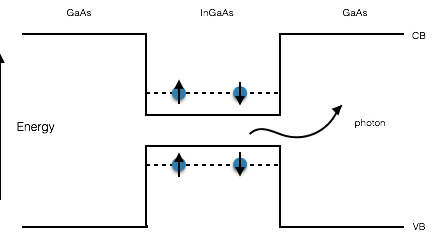
\includegraphics[width=0.7\textwidth]{images/biexciton.png}
    \caption{Energetic structure of the biexciton}
    \label{fig:biexciton}
\end{figure}

Electrons and holes are created in or near the dot by electro- or
photo-excitation. Electrons are excited into the conduction band and
holes are left in the valence band. An e-h pair is referred to as an
exciton. Typically, mobile carriers are created in the bulk material by
above band excitation and they relax into different confinement
potentials in the heterostructure. The QD will normally be the lowest
energy confinement. This scheme is useful because it allows the dot to
be populated by lasers at a lower wavelength than the dot emission
wavelength. Thus the exciting laser and dot are spectrally separated and
can be identified experimentally.

Several excitonic complexes can form inside the QD. A single e-h pair is
an exciton, a double e-h pair is a biexciton. An unbalance in the number
of electrons and holes can cause charge excitonic complexes. For example
a single electron and two holes creates an exciton with an extra hole in
the dot, this is referred to as a positively charged exciton, or
positive trion. The photoluminescence spectrum of each complex is
different due to the Coulomb interaction between the carriers. The
spectrum of the entire QD can be made up of many peaks and identifying
each peak can be done by power dependence measurements and/or photon
correlation measurements.

\subsection{Exciton fine-structure and
entanglement.}\label{exciton-fine-structure-and-entanglement.}

An electron has spin $\pm 1/2$ and a heavy hole has spin $\pm 3/2$
(light holes occupy higher energy levels and are ignored in the scope of
this work). Thus an e-h pair, an exciton, confined in the dot has total
angular momentum projected along the $\hat{z}$-axis $M_z$ of $\pm 1$ or
$\pm 2$.

\begin{figure}[h!]
    \centering
    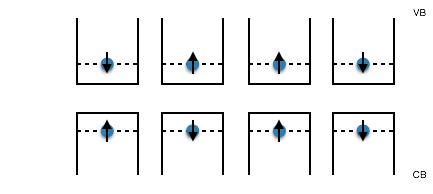
\includegraphics[width=0.7\textwidth]{images/exciton.png}
    \caption{Energetic structure of the exciton, showing the four different spin configurations.}
    \label{fig:exciton}
\end{figure}

Excitons with $M_z = \pm 1$ can optically recombine and are referred to
as bright states. For excitons with $M_z = \pm 2$ optical recombination
is forbidden and are called dark states. Dark states only emit a photon
if a spin flip occurs.

Due to the exchange interaction between the electron and hole, the
fourfold degenerate exciton state, turns into a pair of twofold
degenerate states. One with $M_z = \pm 1$ and one with $M_z = \pm 2$.
The $M_z = \pm 2$ case is energetically lower, due to the aligned spins
of the electron and hole.

The biexciton consists of a pair of anti-aligned electrons and holes, it
thus has no total angular momentum. It is a single degenerate state
because there is no exchange interaction.

Since the total angular moment of the biexciton is zero, it cannot
recombine directly to the ground state, it can only relax to the ground
state through an intermediary state by changing the angular momentum by
$\pm 1$. As the biexciton decays to the exciton an angular momentum
change of $+ 1$ ($-1$) occurs, emitting a right (left) hand circularly
polarised photon. As the exciton then decays to the ground state the
opposite angular momentum change must occur so the change is $-1$($+1$),
emitting a left (right) hand circularly polarised photon. This
transition is shown schematically in Fig
\ref{fig:decaypathsandfinestructure}.

\begin{figure}[h!]
\centering
\begin{subfigure}{.5\textwidth}
  \centering
  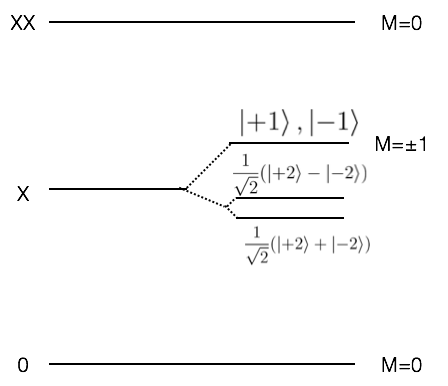
\includegraphics[width=0.8\linewidth]{images/finestructurenofss.png}
  \caption{}
  \label{fig:sub1}
\end{subfigure}%
\begin{subfigure}{.5\textwidth}
  \centering
  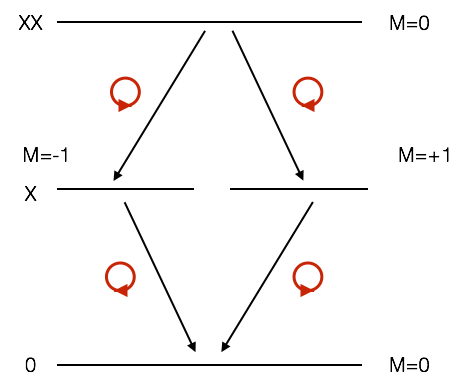
\includegraphics[width=0.8\linewidth]{images/decaypathsnofss.png}
  \caption{}
  \label{fig:decaypath}
\end{subfigure}
\caption{(a) The fine structure of the exciton and (b) the recombination cascade of the biexciton. The biexciton is a singlet state with no angular momentum $M = 0$, the exciton has angular momentum $M = \pm 1$ and the empty dot has $M=0$.}
\label{fig:decaypathsandfinestructure}
\end{figure}

No path is preferential and no which path information can be determined
until a measurement of the emitted photons. The initial electronic state
of the biexciton is that of a singlet state, it is in the superposition
of indistinguishable opposing spin excitons. This entanglement between
the exciton and biexciton should be retained in the emitted photons.
This singlet state can be represented by:

\begin{equation}
\ \left|\psi\right\rangle = \frac{1}{\sqrt{2}} \left(\left|\uparrow\downarrow\right\rangle + \left|\downarrow\uparrow\right\rangle \right).
\end{equation}

After emission the state is in the superposition of the left and right
circularly polarised photons, giving rise to photon polarization
entanglement:

\begin{equation}
\ \left|\psi\right\rangle = \frac{1}{\sqrt{2}} \left(\left|L_{XX} R_X\right\rangle + \left|R_{XX} L_X\right\rangle \right).
\end{equation}

Which is equivalent to

\begin{equation}
\ \left|\psi\right\rangle = \frac{1}{\sqrt{2}} 
\left(\left|H_{XX} H_X\right\rangle + \left|V_{XX} V_X\right\rangle \right).
\end{equation}

In the rectilinear basis (H (V) - horizontal (vertical) polarised
photon). This recombination cascade is presented schematically in Figure
\ref{fig:decaypathsandfinestructure}. This state is one of the maximally
entangled Bell states $\ \left|\Psi^{+}\right\rangle$.

\subsection{Fine structure splitting.}\label{fine-structure-splitting.}

In real QD systems however, the degeneracy of the bright exciton state
is lifted due to a multitude of effects. If the confinement potential
symmetry is low then e-h exchange interaction causes the exciton level
to split.

\begin{figure}[h!]
\centering
\begin{subfigure}{.5\textwidth}
  \centering
  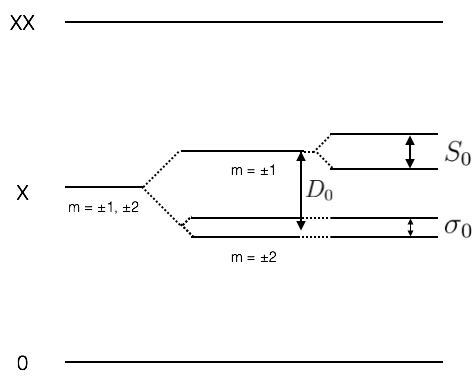
\includegraphics[width=0.9\linewidth]{images/finestructurewithfss.png}
  \caption{}
  \label{fig:sub1}
\end{subfigure}%
\begin{subfigure}{.5\textwidth}
  \centering
  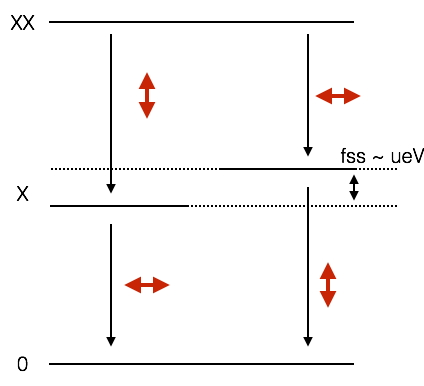
\includegraphics[width=0.9\linewidth]{images/decaypathswithfss.png}
  \caption{}
  \label{fig:decaywithfss}
\end{subfigure}
\caption{(a) The fine structure of the exciton with lifted degeneracy and (b) the two optical decay paths when the dot exhibits fine structure splitting.}
\label{fig:withfss}
\end{figure}

This loss of symmetry can be causes by elongation of the QD, strain,
random alloy segregation or piezoelectric fields in the vicinity of the
dot. When this degeneracy lifting occurs the non-degenerate exciton
levels are split by an energy amount called the fine-structure splitting
(FSS). For the biexciton state e-h exchange interaction does not occur
and it remains a single state. Since the biexciton cascade must
propagate through the exciton state, and there is time evolving mixing
of the exciton non-degenerate levels. This new cascade is shown in
Figure \ref{fig:withfss}. With respect to the emitted photons, the FSS
modifies the entanglement \cite{entangletime}. The biexciton cascade
proceeds as follows. The dot is first populated with a biexciton:

\begin{equation}
\ \left|\psi\right\rangle = \frac{1}{\sqrt{2}} \left(\left|XX_{H} X_H\right\rangle + \left|XX_{V} X_V\right\rangle \right).
\end{equation}

When the biexciton decays to the exciton state, a photon is emitted of
horizontal (H) or vertical (V) polarisation. The QD state becomes a
superposition of the emitted biexciton photon and the exciton remaining
in the dot. The non-degenerate exciton states evolve at different rates,
the difference being proportional to the size of the FSS. The state is
then:

\begin{equation}
\ \left|\psi\right\rangle = \frac{1}{\sqrt{2}} 
\left(\left|H_{XX} X_H\right\rangle + \mathrm e ^{\frac{i FSS \ t}{\hbar}}\left|V_{XX} X_V\right\rangle \right).
\end{equation}

The phase rotates the state until the exciton is emitted after time
$\tau_\Delta$. The final emitted photonic state is then:

\begin{equation}
\ \left|\psi\right\rangle = \frac{1}{\sqrt{2}} 
\left(\left|H_{XX} H_X\right\rangle + \mathrm e ^{\frac{i FSS \ \tau_\Delta}{\hbar}}\left|V_{XX} V_X\right\rangle \right).
\end{equation}

The biexciton and exciton emission lifetimes vary according to decaying
exponential distributions and as such so will $\tau_\Delta$. When the
FSS of the QD is non-zero this varying term $\tau_\Delta$ can cause the
phase of the state to average out to zero, and thus measurements of the
state will look non-entangled.

Entanglement measurements are evaluated on an ensemble of identical
states. In the regime of non-zero FSS however, the state is still
entangled, the states are not identical, and the phase term changes in
each occurrence of emitted pairs. In measurements the overall state
looks mixed with the entanglement degraded. Good entanglement detection
therefore depends on the parameter
$\mathrm e ^{\frac{i FSS \tau_\Delta}{\hbar}}$. If we can make the FSS
to be zero or almost zero therefore we can approach the regime of ideal
entanglement. Much research has gone into quantum dot systems that
control or minimise the FSS \cite{ry1, ry2}. However creating QDs with
perfect zero FSS is difficult.

Another approach would be to select only the emitted photons where
$\tau_\Delta$ is at a pre-determined value \cite{entangletime}. In this
case we can select pairs with a certain phase. This method is called
time-tagging. In theory we can time-tag to prefer multiple maximally
entangled states, for example
$\frac{1}{\sqrt{2}}  \left(\left|H H\right\rangle \pm \left|VV\right\rangle \right)$,
or
$\frac{1}{\sqrt{2}}  \left(\left|H H\right\rangle \pm i\left|VV\right\rangle \right)$.
Selecting different states however is done at the cost of lower
intensity due to the exciton lifetime decaying with exponentially
decaying intensity.

\newpage
\section{Methods}

In this chapter the manufacturing and experimental methods used to
create and categorise the QD's are documented. It should be noted that
the author of this report focused exclusively on the experimental and
theoretical work, and did not manufacture any of the samples. The
manufacturing is described for understanding and also to present the
advantages of the site controlled system.

\subsection{Sample preparation.}\label{sample-preparation.}

In this section the manufacturing methods for the site controlled system
will be documented. The advantage of this system is precise control of
parameters of the grown QD's. The manufacturing steps are also
compatible with existing semiconductor foundry techniques.

\paragraph{Prepatterning.}\label{prepatterning.}

The GaAs (111)B substrates are prepatterned with inverted pyramids by
typical UV lithography and wet chemical etching procedures. A thin layer
of SiO$_2$ and photoresist are layered on the top of the substrate. The
triangular pattern is then transferred from a chrome mask to the
photoresist by exposure to a UV lamp and development in a MF-319
solution. This pattern is transferred to the SiO$_2$ using hydrofluoric
acid. A Br:Methanol solution is used to etch into the GaAs, where the
anisotropy of the etch between the (111)A and (111)B surfaces results in
the inverted pyramid being inserted into the substrate. The profile of
the substrate is now of a periodic array of inverted pyramids. Peak to
peak distance between pyramids is 7.5$\mu$m.

\paragraph{MOVPE Growth.}\label{movpe-growth.}

The semiconductor layers were grown on the patterned substrate by
Metalorganic vapour phase epitaxy (MOVPE). MOVPE growth is complex and
will not be described in detail here. The epitaxial layers grown is as
follows:

\begin{enumerate}
\def\labelenumi{\arabic{enumi}.}
\itemsep1pt\parskip0pt\parsep0pt
\item
  A think GaAs buffer layer.
\item
  A protective $\text{Al}_{0.75}\text{Ga}_{0.25}\text{As/GaAs}$ layer.
\item
  Double barrier structures of
  $\text{Al}_{0.55}\text{Ga}_{0.45}\text{As/GaAs}$.
\item
  GaAs.
\item
  Active $\text{In}_x\text{Ga}_{1-x}\text{As/GaAs}$ layer.
\end{enumerate}

\begin{figure}[h!]
\centering
\begin{subfigure}{.5\textwidth}
  \centering
  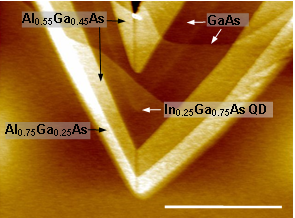
\includegraphics[width=1\textwidth]{images/layers.png}
  \caption{}
  \label{fig:sub1}
\end{subfigure}%
\begin{subfigure}{.5\textwidth}
  \centering
  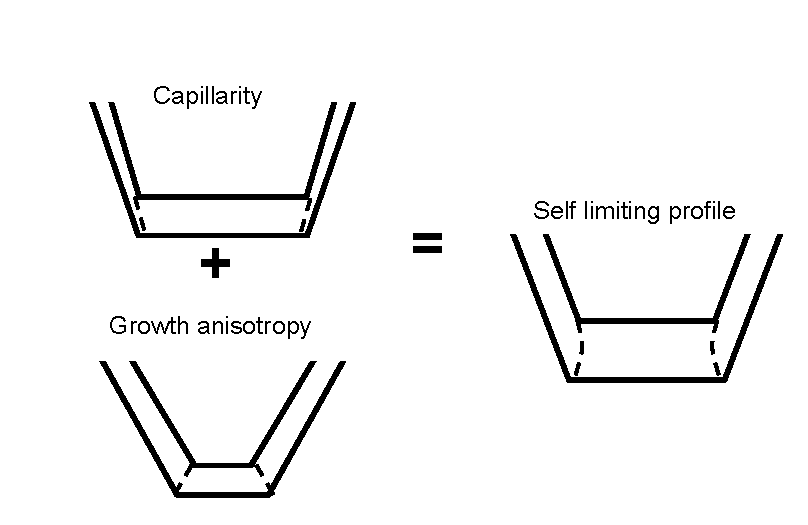
\includegraphics[width=1\textwidth]{images/selflim.pdf}
  \caption{}
  \label{fig:decaypath}
\end{subfigure}
\caption[]{(a)  AFM image\protect\footnotemark  of a cleaved pyramid showing the epitaxially grown semiconductor layers. (b) Self limiting profile formation that gives rise to the QD shape at the tip of the pyramid caused by the capilariy and growth anisotropy effects described in the text.}
\label{fig:afmlayers}
\end{figure}

\footnotetext{Courtesy of the EPN group.} An AFM image of these layers
is shown in Figure \ref{fig:afmlayers} (a). QDs are self-formed at the
central axis of the $\text{In}_x\text{Ga}_{1-x}\text{As/GaAs}$ layer.
The properties of the QD growth depend on the equilibrium of the growth
anisotropy and capillarity effects. Growth anisotropy is due to the
differing growth rates on the (111)A surface on the faces of the
pyramids and the (111)B surface at the bottom, it increases the growth
rate on the pyramid faces. The capillarity effect is due to adatoms
diffusing to reduce surface energy by increasing planarity, thus the
tend to diffuse to the bottom of the pyramid, it increases the growth
rate at the bottom (the tip in the apex down geometry) of the pyramid.
The equilibrium of these process gives rise to the self limiting profile
of the QD layer. This is shown schematically in Figure
\ref{fig:afmlayers} (b).

The advantage of the MOVPE growth is that the self limiting profile that
dictates the QD shape and size, which in turn change the emission
wavelength and exciton-biexciton binding energy etc., can be altered by
changing growth temperature and alloy composition.

\subparagraph{Surface etching.}\label{surface-etching.}

The pyramids are still in the apex down geometry. The surface etching is
primarily to increase the quality of the emission spectrum, some
irregularities that form at the top of the sample can be confusing in
the optical spectrum. The sample is layered with photoresist, then
oxygen plasma partially etches away the photoresist until the
irregularities are uncovered but photoresist remains in the pyramid. The
irregularities are then etched away with sulfuric acid and peroxide.

\subparagraph{Back etching.}\label{back-etching.}

This procedure `flips' the pyramids into a free standing apex up
geometry. The pyramid acts as a lens that decreases internal reflections
and the and enhances the emission collection by up to three orders of
magnitude. The lens gives the emitted photons a preferential `up'
direction towards the collection aperture. Another support substrate is
prepared with strips of titanium and gold on the surface. A titanium and
gold layer is evaporated onto the original sample.

\begin{figure}[h!]
    \centering
    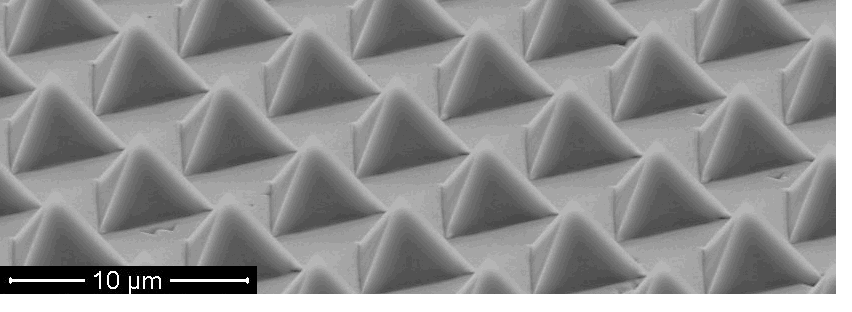
\includegraphics[width=.5\textwidth]{images/sem.png}
    \caption{SEM image\protect\footnotemark  of the free standing pyramids after back etching.}
    \label{fig:sem}
\end{figure}

\footnotetext{Courtesy of the EPN group.}

The two substrates are attached thermo-compression gold bonding. The
strips allow air to escape when the sample is cooled to $\sim$ 8K. The
original substrate is etched away by different chemical solutions. The
etching rate of the $\text{Al}_{0.75}\text{Ga}_{0.25}\text{As/GaAs}$
layer on the pyramid is much slower than that of GaAs, so that the QD
layers are protected. An scanning electron microscopy image of these
free standing pyramids is shown in Figure \ref{fig:sem}.

\subsection{Spectroscopy.}\label{spectroscopy.}

Optical characterisation of single pyramids is done with a standard
micro photoluminescence setup (see Figure \ref{fig:upl}). A continuous
wave (cw) laser diode ($\lambda$=658nm) or pulsed laser diode
($\lambda$=650nm) can be used to excite the QD. The cw laser allows
higher emission intensity because the QD is immediately repopulated
after relaxation. The pulsed laser is used for time-resolved
measurements. High magnification (100x) of the sample surface is
achieved using a small working distance of the objective. The laser beam
is focused to a point on the sample smaller that the area of a single
pyramid. Before the QD emission is sent to the spectrometer the laser
light is filtered by a long-pass filter. The filtered emission is then
sent to the spectrometer equipped with a charge-coupled device (CCD) or
InGaAs detector array.

\begin{figure}[h!]
    \centering
    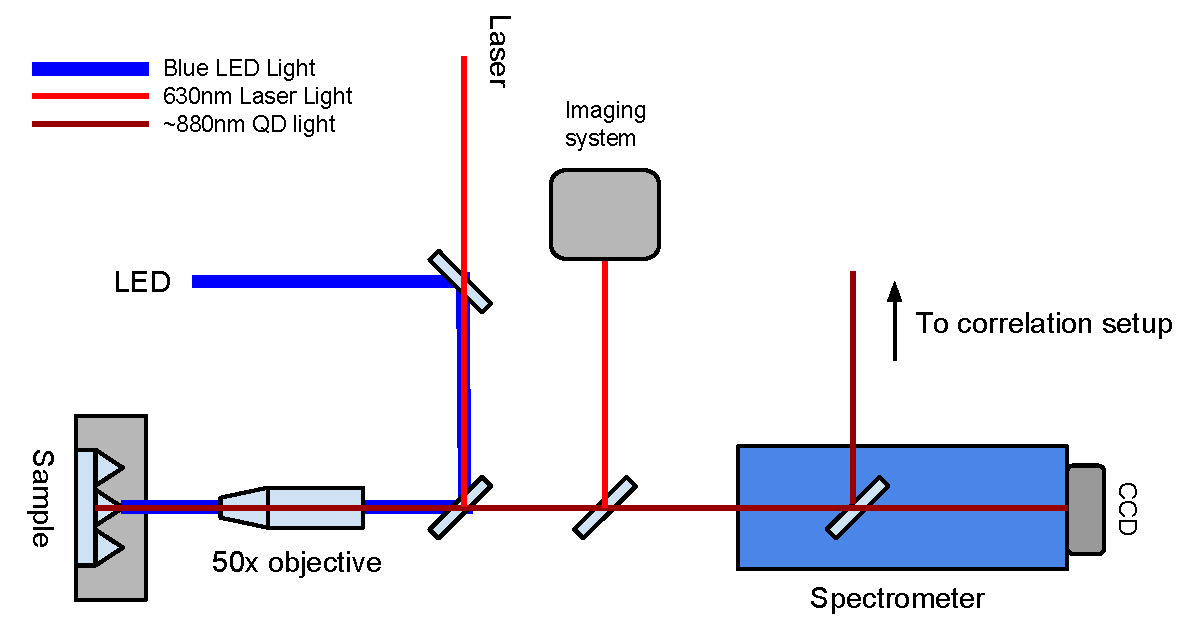
\includegraphics[width=0.8\textwidth]{images/PL.pdf}
    \caption{Schematic of the micro photoluminescence setup.}
    \label{fig:upl}
\end{figure}

The sample is mounted in a closed-cycle helium cryostat and the
temperature used for measurement is typically 8K. A blue LED can be used
to illuminate the sample. By placing a beamsplitter in the optical axis
the image of the sample surface is sent to the CCD. This allows
simultaneous imaging of the sample surface and measurement of the
photoluminescent spectrum. This is typically used to find a candidate QD
for further measurements. The beamsplitter is removed during
measurements to increase collection efficiency.

Measurements of the FSS were carried out by placing a half-wave plate
and a linear polarizer in-line with the emission axis, between the QD
source and spectrometer. The FSS causes the energetic/spectral positions
of the exciton and biexciton transitions follow counter phase sinusoids
while changing polarization angle. The sinusoidal curve is obtained by
subtracting the biexcitons energy from the excitons. The amplitude of
the sinusoid has the value of FSS.

For time-resolved measurements such as measuring the lifetimes and
correlations avalanche photo diodes (APDs) and photon counting modules
(PCMs) are used. The spectrometer can work as a monochromator and an
internal lateral mirror sends the selected wavelength through an exit
slit towards the APDs. APDs can detect single photons and are synced
with the PCM to give the arrival time of the photons in the lifetime
measurements. The histogram of such arrival times gives the
photoluminescent decay curves from which the state lifetime can be
determined.

\subsection{Photon correlation
measurements.}\label{photon-correlation-measurements.}

\begin{figure}[h!]
    \centering
    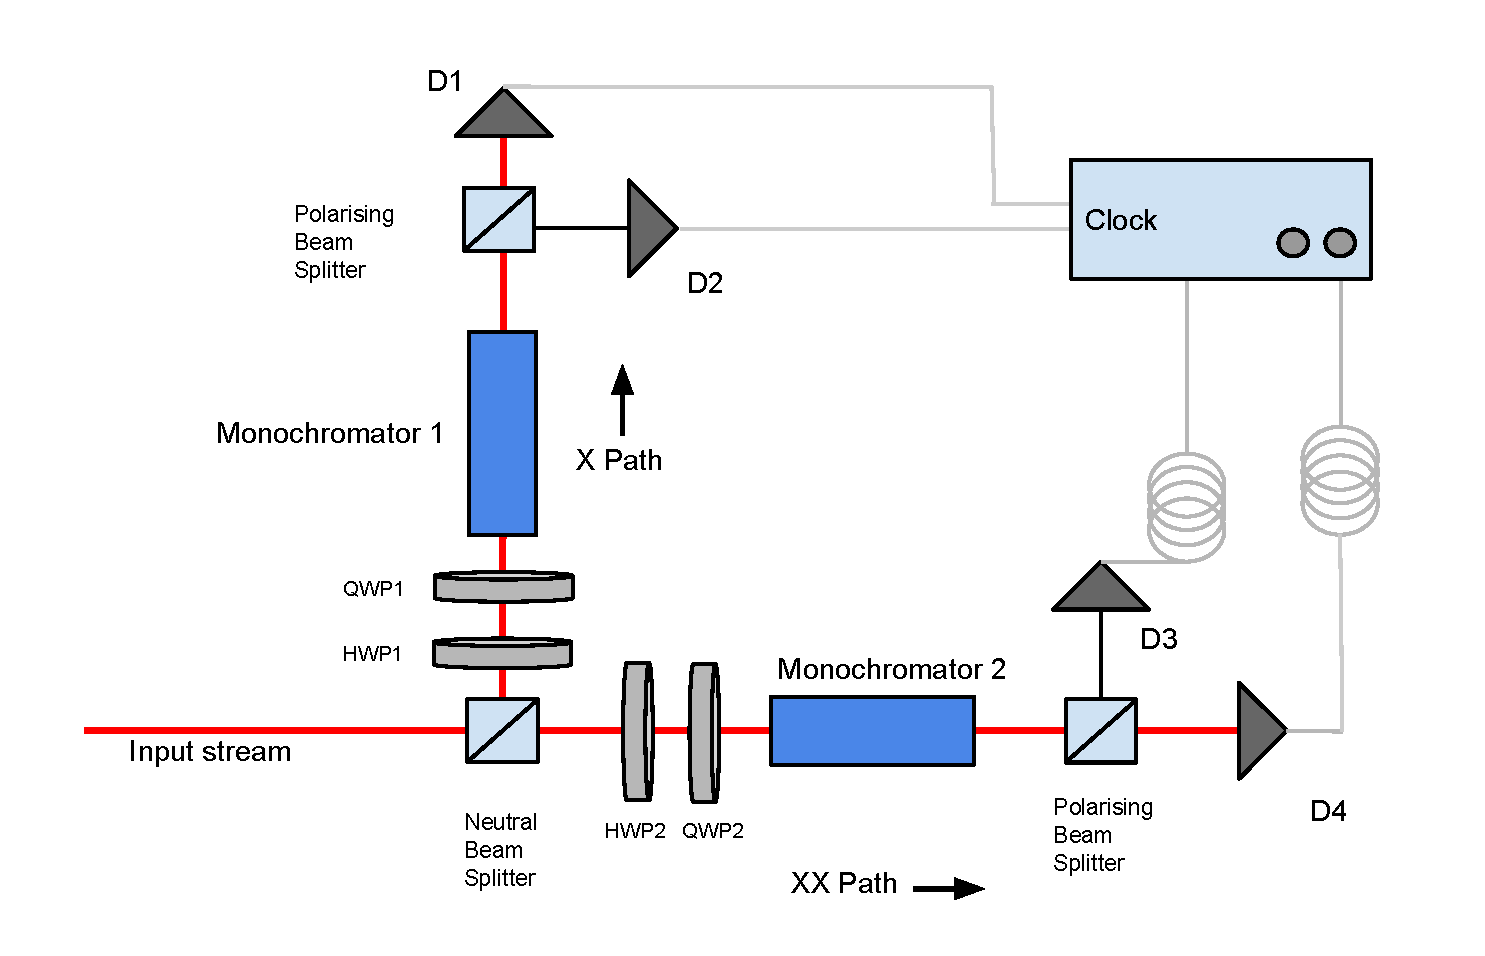
\includegraphics[width=0.8\textwidth]{images/hbt.pdf}
    \caption{Schematic of the Hanbury Brown Twiss correlator.}
    \label{fig:hbt}
\end{figure}

Polarisation resolved correlation measurements are carried out in a
Hanbury Brown and Twiss (HBT) setup. The experiment schematic is
presented in Figure \ref{fig:hbt}. The QD emission stream is sent
towards a non-polarising 50:50 beam splitter. A polarisation projection
is chosen using a combination of half and quarter waveplates. The
exciton and biexciton photons are energetically different and they
discriminated using monochromators. Each filtered photon was selected by
a polarizing beamsplitter and sent to avalanche photodiodes detectors
(APDs). Two APDs are used in each channel, one starts a counting module,
the other stops it. The stop event is electrically delayed in order to
obtain negative correlation values. The obtained curves represent the
second order correlation function $g^{(2)}(\tau)$ (see Ref. \cite{fox}
for a good introduction).

\begin{equation}
g_{ij}^{(2)}(\tau) = \frac{\left\langle I_i(t)I_j(t+\tau) \right\rangle}{\left\langle I_i(t) \right\rangle \left\langle I_j(t+\tau) \right\rangle}
\end{equation}

Where $I_n(t)$ is the intensity of state $n$ at time $t$.
$g^{(2)}(\tau)$ represents the conditional probability of a $j$-th
excitonic transition photon to be measured at the time $\tau$ after the
$i$-th excitonic transition photon is measured. Four synchronized
sequences of detector signals were used to build four correlation
curves. By choosing different polarisation bases (Typically rectilinear,
diagonal and circular) and measuring $g^{(2)}(\tau)$, the
biexciton-exciton photon entanglement can be chategorised. The degree of
correlation in each basis can be calculated by
$C = \frac{ g^{(2)}_{\parallel}(0) - g^{(2)}_{\perp}(0) }{ g^{(2)}_{\parallel}(0) + g^{(2)}_{\perp}(0) }$.
Where $g^{(2)}_{\parallel}(\tau)$ is the $g^{(2)}$ value for
co-polarised pairs and $g^{(2)}_{\perp}(\tau)$ for cross-polarised
pairs. $g^{(2)}(0)$ is the integrated number of events in the central
peak. From these values the fidelity to the
$\frac{1}{\sqrt{2}} \left(\left|H_{XX} H_X\right\rangle + \left|V_{XX} V_X\right\rangle \right)$
state can be calculated by $F = \left(1 + C_R + C_D - C_C \right)/4$.
This fidelity value is readily accepting by the scientific community as
an evaluation of entanglement \cite{f1, entandiode}. It is also much
quicker to measure the fidelity, which requires measurements in 3 bases,
than to do a full photonic state tomography procedure, which requires 16
basis measurements \cite{amotomo}.

\subsection{Modelling the experiment.}\label{modelling-the-experiment.}

The simulation\cite{self2, github} attempts to realistically model the
single photon correlation curves and polarization resolved correlation
curves from a semiconductor quantum dot. A monte carlo simulation of the
QD was combined with a model of the optical bench, this allows a monte
carlo simulation of the experiment and of various results such as the
polarisation resolved correlation curve or photonic state tomography
\cite{amotomo}.

\paragraph{Quantum dot Monte Carlo.}\label{quantum-dot-monte-carlo.}

This monte carlo model simulates the QD emission properties, namely, its
emission probabilities related to the excitation laser or current and
its emission time statistics. For the polarization resolved curves fine
structure splitting and decoherence effects were also taken into
account. The Poisson photon emission probability of the quantum dot
after excitation by a laser or a voltage are \cite{grundmann}

\begin{align} 
p_x(n) &= 1 - e^{- n}\\
p_{xx}(n) &= 1 - (1+n)e^{- n}
\end{align}

Where $p_x$ and $p_{xx}$ are the probabilities of exciton and biexciton
emission respectively, $n$ is the mean number of generated excitons in
the bulk/vicinity of the dot. These are assumed, and will naturally give
rise to the typical single and cross correlation curves in pulsed
excitation mode.

The exciton and biexciton lifetimes are randomly chosen from an
exponential decay with characteristic lifetime $\tau_x$ and $\tau_{xx}$
respectively. The characteristic lifetime of the biexciton is typically
around half that of the exciton. It is made sure in the simulation that
the specific biexciton emission lifetime is always shorter than that of
the exciton.

In the polarization resolved case a biphoton state is emitted. This is
represented by

\begin{equation} 
\left|\psi\right\rangle = \left|H_xH_{xx}\right\rangle + e^{i FSS \  \tau/\hbar}\left|V_xV_{xx}\right\rangle
\end{equation}

The phase term is given by $e^{i FSS \ \tau/\hbar}$ where $FSS$ is the
fine structure splitting and $\tau$ is the time between the biexciton
and exciton emission. In the perfect case of no fine structure splitting
the phase term will always be 1.

Decoherence must also be taken into account, this is a process whereby
the phase term randomly shifts. Here it is phenomenologically
categorised by a characteristic cross decoherence time of $\tau_{HV}$.
It is reported that this time $\tau_{HV}$ is typically\cite{hudson}
longer that the exciton lifetime, implying that QD excitons have a
coherence \textgreater 70\%, i.e.~70\% of the time the emission will not
have a random phase shift.

\paragraph{Modelling the optical
bench.}\label{modelling-the-optical-bench.}

A model of the optical elements includes mathematically writing the
photonic state in an algebraic lab basis and by using Jones tensor
algebra\cite{bible, jones} the state can be propagated through the
optical bench. The degrees of freedom in this basis are photonic
polarization, direction and energy. Polarization is needed since the
photons from the quantum dot should be polarization entangled. Direction
is needed in order to tell the difference between the output paths of a
polarising beam splitter (PBS) and a neutral beam splitter (NBS). Energy
is needed to differentiate between the exciton and biexciton state.

The polarisation basis is given by\cite{jones1}:

\begin{equation}
\hat{h} = \begin{pmatrix}1\\0\end{pmatrix}, \hat{v} = \begin{pmatrix}0\\1\end{pmatrix}
\end{equation}

The direction basis is given by:

\begin{equation}
\hat{i} = \begin{pmatrix}1\\0\end{pmatrix}, \hat{j} = \begin{pmatrix}0\\1\end{pmatrix}
\end{equation}

The energy basis is given by:

\begin{equation}
\hat{e}_x = \begin{pmatrix}1\\0\end{pmatrix}, \hat{e}_{xx} = \begin{pmatrix}0\\1\end{pmatrix}
\end{equation}

For example, an input photon that is $\hat{h}$ polarized, moving in the
x direction and with energy $\hat{e}_x$ is calculated by:
$\gamma_{eg} = \hat{h} \otimes \hat{i} \otimes \hat{e}_x$, where
$\otimes$ is the tensor product operator.

These basis matrices are used to categorise matrix operators for various
optical bench apparatus, namely the neutral and polarising beam
splitters and monochromators. The matrix operators can be found by
mapping each of the input states to the output states \cite{bible}.

\begin{equation}
M = \sum_{i} \left| \text{in}_i \right\rangle \left\langle \text{out}_i\right| 
\end{equation}

The input and output states and matrix operators are presented in
Appendix A for the neutral and polarising beam splitters and
monochromators. For the wave plates, rotated at an angle $\theta$ to the
optical axis, the common Jones matrices are used \cite{jones2}.

\begin{equation}
HWP = \begin{pmatrix} \cos{2 \theta} & \sin{2 \theta} \\ \sin{2 \theta} & -\cos{2 \theta} \end{pmatrix}
\end{equation}

\begin{equation}
QWP = \begin{pmatrix} 1 + i \cos{2 \theta} & i \sin{2 \theta} \\ i \sin{2 \theta} & 1- i \cos{2 \theta} \end{pmatrix}
\end{equation}

These are then adapted to the lab basis. The adapted matrices derived
for the PBS (polarising beam splitter), S (monochromator), NBS (neutral
beam splitter), QWP and HWP are presented in Appendix A. The detector
matrices are simply given by the photonic state that the detector is
allowed measure, for example Detector1 in Figure \ref{fig:hbt} is only
able to measure $\hat{h}$ polarized photons with energy $\hat{e}$ moving
in the $\hat{i}$ direction.

\begin{align}
D1 &= \hat{h} \otimes \hat{i} \otimes \hat{e}_x\\
D2 &= \hat{v} \otimes \hat{i} \otimes \hat{e}_x\\
D3 &= \hat{h} \otimes \hat{i} \otimes \hat{e}_{xx}\\
D4 &= \hat{v} \otimes \hat{j} \otimes \hat{e}_{xx}
\end{align}

All of the matrices defined here act on a single photon state. In the
entangled photon case each of this matrices are modified by the
relation\cite{rioux}

\begin{equation}M_{e} = M \otimes M\end{equation}

The total optical bench operator is then given by

\begin{equation}
L_e = PBS_e \cdot S_e \cdot QWP_e \cdot HWP_e \cdot NBS_e
\end{equation}

The detector pair matrices are given by

\begin{equation}
D_iD_j = D_i \otimes D_j
\end{equation}

The pairs D1D3, D1D4, D2D3, D2D4 are always used. We can then find what
the probability of a given input state $\left|\psi\right\rangle$ will
have of hitting a detector pair $D1D3$ is given by

\begin{equation}
P_{D1D3} = |D1D3^{T} \cdot L_e \cdot \left|\psi\right\rangle |^2
\end{equation}

\paragraph{The simulation algorithm}\label{the-simulation-algorithm}

The simulation starts by generating the photonic state
$\left|\psi\right\rangle = \left|H_xH_{xx}\right\rangle + e^{i S \tau/\hbar}\left|V_xV_{xx}\right\rangle$
in the lab basis

\begin{equation}
\left|\psi\right\rangle = \left| (\hat{h} \otimes \hat{i} \otimes \hat{e}_x) \otimes(\hat{h} \otimes \hat{i} \otimes \hat{e}_{xx}) \right\rangle + e^{i S \tau/\hbar}\left|(\hat{v} \otimes \hat{i} \otimes \hat{e}_x) \otimes(\hat{v} \otimes \hat{i} \otimes \hat{e}_{xx})\right\rangle
\end{equation}

The lifetime is generated and the phase calculated, if a decoherence
event happens before the lifetime is finished, the phase is shifted by
some random amount. The state is the operated on by the lab matrix and
the detector pair probabilities are calculated. Then stochastically, a
single detector, or pair of detectors were chosen according to these
probabilities. Tagging each detector with a hit time according to the
lifetime and laser pulse interval of the exciton or biexciton the
polarisation resolved correlation curves are generated. These curves can
be generated in different polarisatoin bases by changing the waveplate
angles.

\newpage
\section{Time resolved entanglement}

The theoretical and experimental work to validate the idea of time
dependent entanglement is discussed in this chapter. This work was done
by the author and Dr.~Gediminas Juska, both took measurements and both
worked on the processing.

\subsection{Theory of time gating.}\label{theory-of-time-gating.}

As explained in Chapter 1 the entangled photonic state from the QD is
predicted to be\cite{entangletime}:

\begin{equation}
\ \left|\psi\right\rangle = \frac{1}{\sqrt{2}} 
\left(\left|H_{XX} H_X\right\rangle + \mathrm e ^{\frac{i FSS \ \tau_\Delta}{\hbar}}\left|V_{XX} V_X\right\rangle \right).
\end{equation}

Where $\tau_\Delta$ is the time between biexciton and exciton photon
emission and $FSS$ is the exciton fine structure splitting. If the FSS
is large enough this phase oscillation becomes fast and when averaged
over all QD emissions with $\tau_\Delta$ obeying an exponential
distribution, the phase will average out to zero. The state is still
entangled, however each emitted pair is different and under measurement
will seem to be classical light.

\begin{figure}[h!]
    \centering
    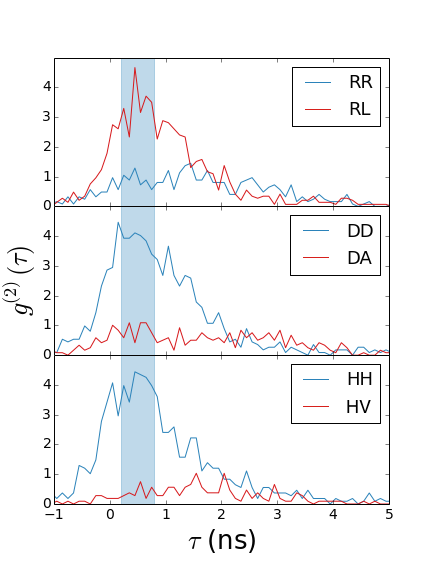
\includegraphics[width=0.5\textwidth]{notebooks/correlations_gate.png}
    \caption{A simple gate applied to the central peak of the correlation curve shown in Figure \ref{fig:correlationsdata}.}
    \label{fig:timegateschematic}
\end{figure}

Since it is not feasible to change the FSS of each emission, we instead
discriminate the data based on $\tau_\Delta$. We choose only small
$\tau_\Delta$ in the correlation curves by applying a time gate. This
time gate is shown schematically in Figure \ref{fig:timegateschematic}.

Consider a gate that starts at time $t_0$ and has a width $\Delta t$.
For $t_0 = 0$ and $\Delta t \to 0$ we would expect the maximally
entangled state

\begin{equation}
\ \left|\psi\right\rangle = \frac{1}{\sqrt{2}} 
\left(\left|H_{XX} H_X\right\rangle + \left|V_{XX} V_X\right\rangle \right).
\end{equation}

Decoherence\cite{hudson} will reduce the measurable fidelity to this
state to some value $F_{max} \leq 1$. In practice the gate must have
some nonzero finite width. If $t_0$ is kept constant and the $\Delta t$
is increase it would be expected that the fidelity will drop as photon
pairs with a different $\tau_\Delta$ are included in the calculation.
The biphoton intensity will increase for larger $\tau_\Delta$. If
$\Delta t$ is kept constant and $t_0$ is increased it would be expected
that the fidelity will vary sinusoidally synchronised with the state
phase. If the measured fidelity is plotted versus the gate start time
for an adequately small $\Delta t$ it should be possible to derive an
accurate estimation of the FSS.

In theory by choosing vanishingly small $\Delta t$ is would be possible
to prepare an entangled state with every conceivable phase. In practice
however since the biexciton and exciton lifetimes are exponentially
decreasing, the emission intensity is exponentially decreasing as $t_0$
increases.

\subsection{Experimental data.}\label{experimental-data.}

In Figure \ref{fig:correlationsdata} is shown the measured correlation
curves in linear, diagonal and circular bases. In this measurement the
time resolution was 0.1 $ns$ which is considered to be high enough for
time gating.

The degree of correlation in each basis can be calculated by
\cite{entandiode}:

\begin{equation}
C = \frac{ g^{(2)}_{\parallel}(0) - g^{(2)}_{\perp}(0) }{ g^{(2)}_{\parallel}(0) + g^{(2)}_{\perp}(0) }
\end{equation}

Where $g^{(2)}_{\parallel}(\tau)$ is the $g^{(2)}$ value for
co-polarised pairs and $g^{(2)}_{\perp}(\tau)$ for cross-polarised
pairs. $g^{(2)}(0)$ is the integrated number of events in the central
peak.

The degree of correlation in linear, diagonal and circular polarisation
bases were calculated to be $C_R = 0.66 \pm 0.06$,
$C_D = 0.46 \pm 0.04$, $C_C = -0.31 \pm 0.02$ respectively.

From these values the fidelity to the
$\frac{1}{\sqrt{2}}  \left(\left|H_{XX} H_X\right\rangle + \left|V_{XX} V_X\right\rangle \right)$
state can be calculated by :

\begin{equation}
F = \frac{1 + C_R + C_D - C_C}{4}.
\end{equation}

The value calculated was $F = 0.61 \pm 0.02$. The errors in the degree
of correlations and the fidelity were calculated by taking the standard
deviation of the same result in the side peaks. The side peaks should
have $C = 0$, and any fluctuations would be due to noise, this noise was
taken to be the error in the results.

The fidelity limit for classical light is $0.5$, the fidelity calculated
from the data beats this limit by over $5$ standard deviations. Clearly
the photons emitted from the quantum dot are exhibiting quantum
behaviour.

When the phase of the photonic state is included into the discussion it
is understood that this fidelity value is the average of all the events
with gate $t_0 \to -\alpha$ and $\Delta t \to \alpha$ where $\alpha$ is
half the time between laser pulses, $\alpha = 6.25 ns$ in the case
presented here.

\begin{figure}[h!]
    \centering
    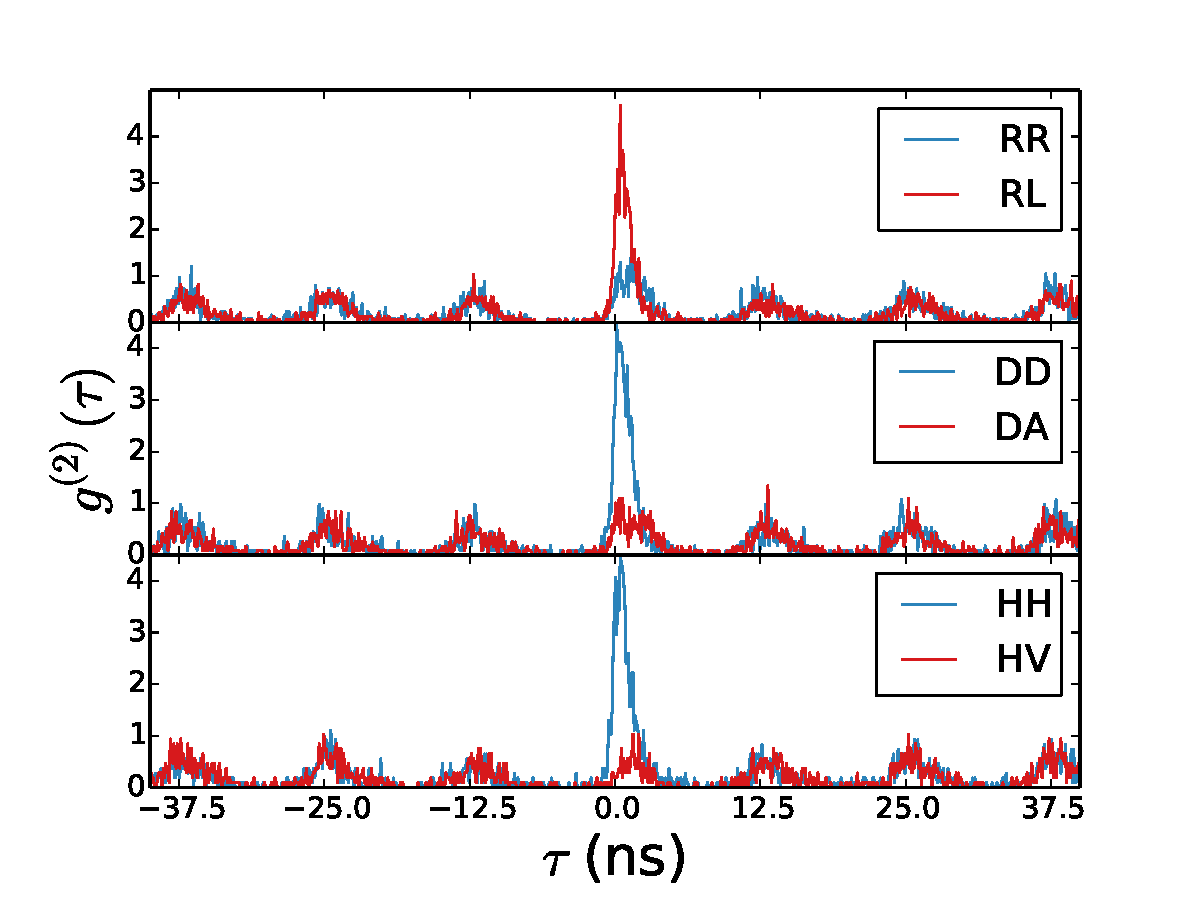
\includegraphics[width=0.7\textwidth]{notebooks/correlations.pdf}
    \caption{Measured correlation curves in the linear, diagonal and circular bases.}
    \label{fig:correlationsdata}
\end{figure}

\subsubsection{Fidelity versus gate start
time.}\label{fidelity-versus-gate-start-time.}

\begin{figure}
\centerfloat
\begin{subfigure}{.5\textwidth}
  \centering
  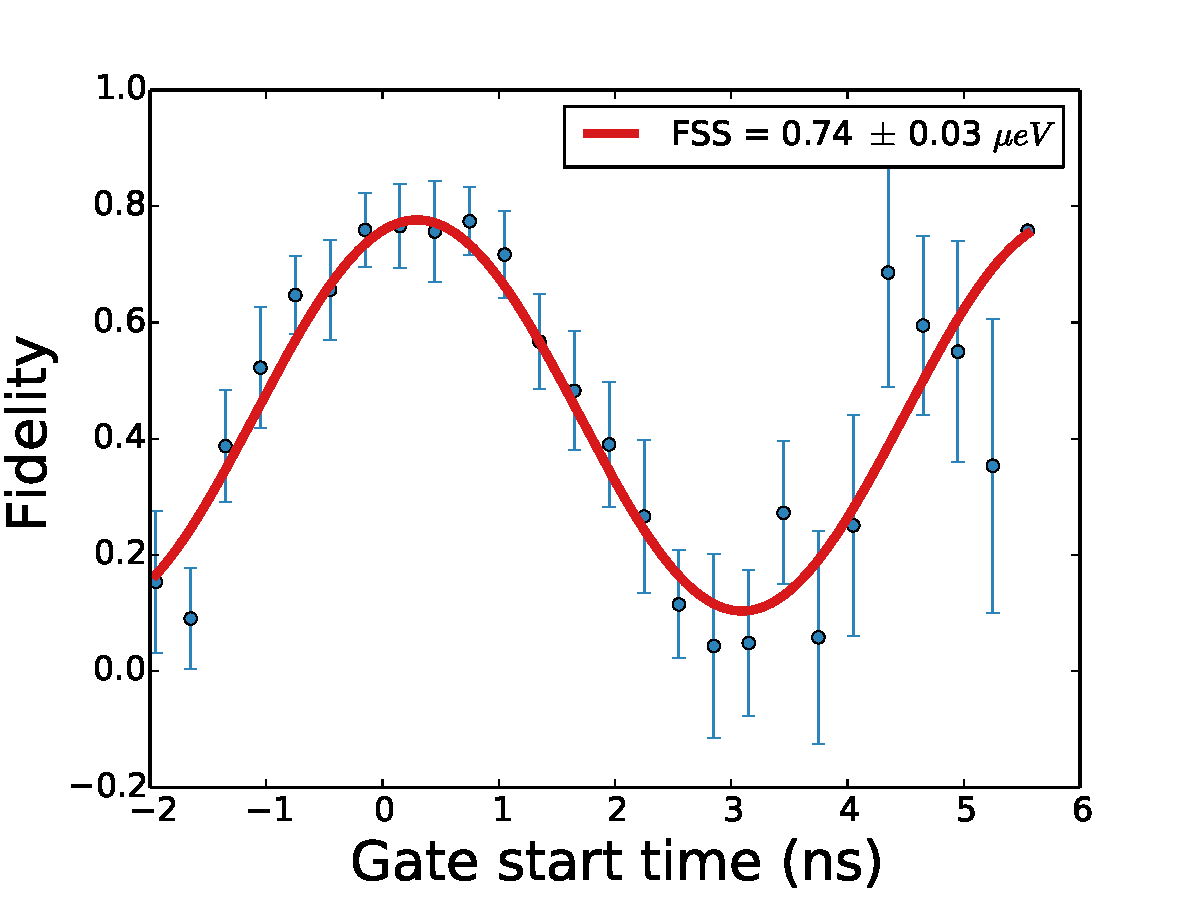
\includegraphics[width=1\linewidth]{notebooks/fidelity_gatestart.pdf}
  \caption{}
  \label{fig:sub1}
\end{subfigure}%
\begin{subfigure}{.5\textwidth}
  \centering
  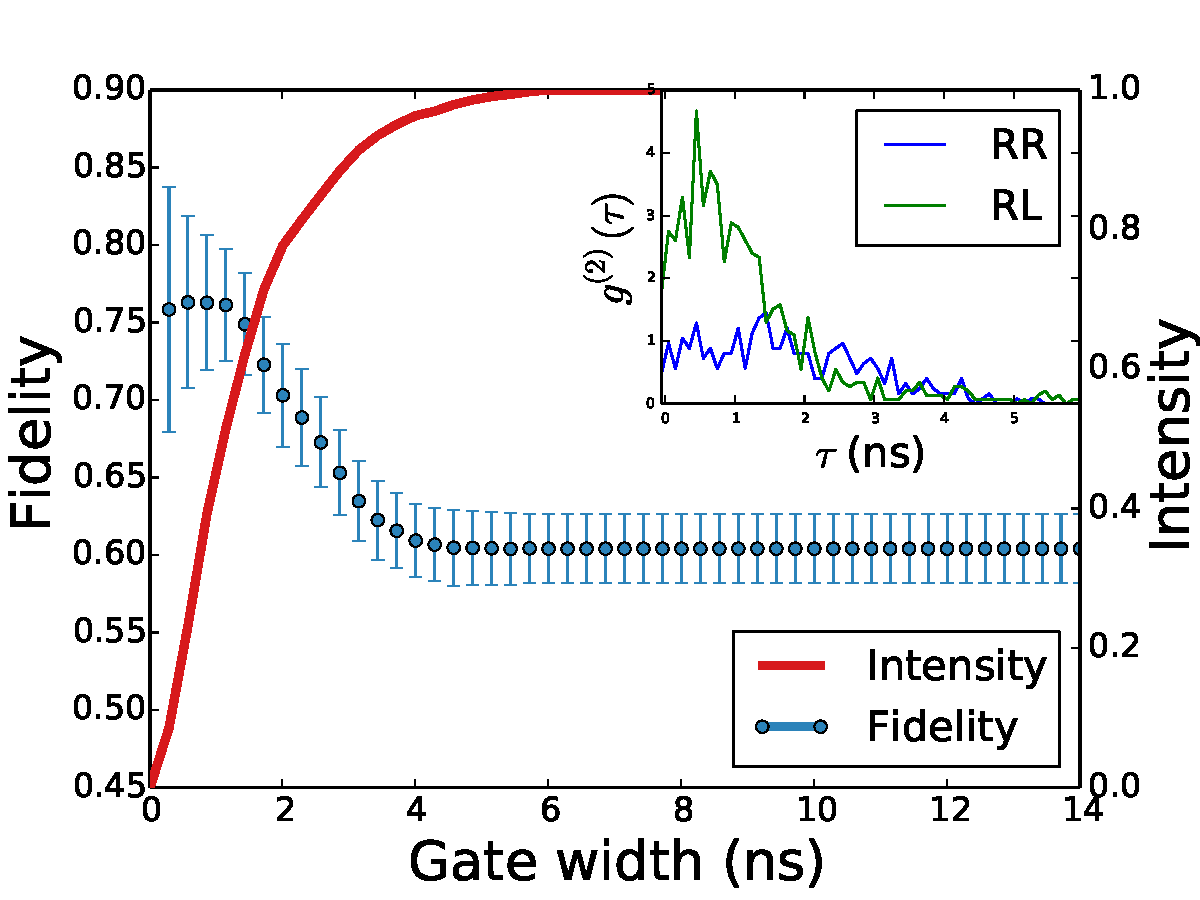
\includegraphics[width=1\linewidth]{notebooks/fidelity_gatewidth.pdf}
  \caption{}
  \label{fig:decaypath}
\end{subfigure}
\caption{(a) Measured fidelity vs gate start for a gate width of 0.2 $ns$ (b) Measured fidelity vs gate width starting at 0 $ns$, the inset shows the section of the curve used.}
\label{fig:timegatedata}
\end{figure}

Figure \ref{fig:timegatedata} presents the results when a gate was
applied to the correlation curves from Figure
\ref{fig:correlationsdata}. First a gate was applied with
$\Delta t = 0.2 ns$ and $t_0 = -2 \to 6 ns$ ($\delta t = 0.2ns$). Figure
\ref{fig:timegatedata} (a) clearly shows a sinusoidal dependence of the
fidelity on $t_0$. The error in the data was again calculated using the
side peaks.

The FSS can be calculated from the curve by fitting a sinusoid and
calculating the frequency. The angular frequency of the fit is
$\nu_f \pm \Delta \nu_f$. We want the term
$\mathrm e^{\frac{i S \tau_\Delta}{\hbar}}$ to oscillate with period
$2\pi$, where $\nu = \frac{1}{\tau_\Delta}$. The result after
substitution is:

\begin{equation}
S = \hbar \nu_f
\end{equation}

The resulting FSS is calculated to be 0.74 $\pm$ 0.03 $\mu eV$. In
Figure \ref{fig:timegatedata} (a) it is seen that the fidelity can rise
to almost 0.8 and drop to less than 0.2, this low value implies
increased fidelity to the state:

\begin{equation}
\ \left|\psi\right\rangle = \frac{1}{\sqrt{2}} 
\left(\left|H_{XX} H_X\right\rangle - \left|V_{XX} V_X\right\rangle \right).
\end{equation}

However there is not enough intensity within this gate to conclusively
show correlation curves for this state. A QD with FSS of around 0.2
\textasciitilde{} 0.3 $\mu eV$ might be better suiting to preparing this
state because the phase oscillations would be slower. However anytime
this state is prepared, it comes at a cost of much reduced intensity.

\subsubsection{Fidelity versus gate
width.}\label{fidelity-versus-gate-width.}

Figure \ref{fig:timegatedata} (b) presents the curve obtained when a
gate was applied to the data with $t_0 = 0ns$ and $\Delta t$ was varied.
It is seen that when $\Delta t$ is small the fidelity is higher, hitting
a high of fidelity of 0.75. As $\Delta t$ is increased, longer time
phase events are included and the fidelity is expected to drop, this is
what we observe. As the gate is opened even more the fidelity drops to a
constant value matching the average fidelity calculated earlier of
$F = 0.61 \pm 0.02$.

It should be pointed out however is the QD's measured in this work, when
a gate is applied that retains 70\% of the intensity a rise in fidelity
from 0.61 to 0.75 can be observed. This would be quite useful in the
future if a physical shutter time gate was used.

The slight plateau in the fidelity at very small values of $\Delta t$ is
attributed to the rise time in the correlation curves near $t_0 = 0ns$.

\subsection{Simulation results.}\label{simulation-results.}

The experimental results presented above were also compared with
theoretical results presented in this section. Using the Monte Carlo
simulation explained in the Chapter 2, the correlation curves were
generated and the time gate processing was applied.

Figure \ref{fig:correlationssim} and Figure \ref{fig:timegatesim} show
these simulated results. Overall there is very good agreement between
the simulations and data.

\begin {table}[h]
\begin{center}
\begin{tabular}{ |l|l| }
  \hline
  \textbf{Parameter} & \textbf{Value} \\\hline
  Exciton lifetime & 2 ns \\\hline
  Biexciton lifetime & 1 ns \\\hline
  Mean excitons in vicinity per pulse & 1 \\\hline
  FSS & 0.7 $\mu eV$ \\\hline
  Decoherence time & $10^6$ ns \\\hline
  Background rate & 15\% \\\hline
  Detector response & 0.3 ns \\\hline
\end{tabular}
\caption{Parameters used to simulate the curves in Figure \ref{fig:correlationssim} and Figure \ref{fig:timegatesim}.}
\label{tab:paramstable}
\end{center}
\end {table}

The simulation takes into account decoherence events, detector response,
FSS, lifetimes, emission intensity and background emission. Many of
these parameters are measurable directly, (FSS, lifetimes, intensity,
detector response) some cannot be measured directly (background and
decoherence). A useful curve that the simulation can predict is the
fidelity versus FSS, which has been shown to be a Lorentzian
\cite{hudson}, however tuning the FSS to measure this curve was outside
the scope of this work.

\begin{figure}[h!]
    \centering
    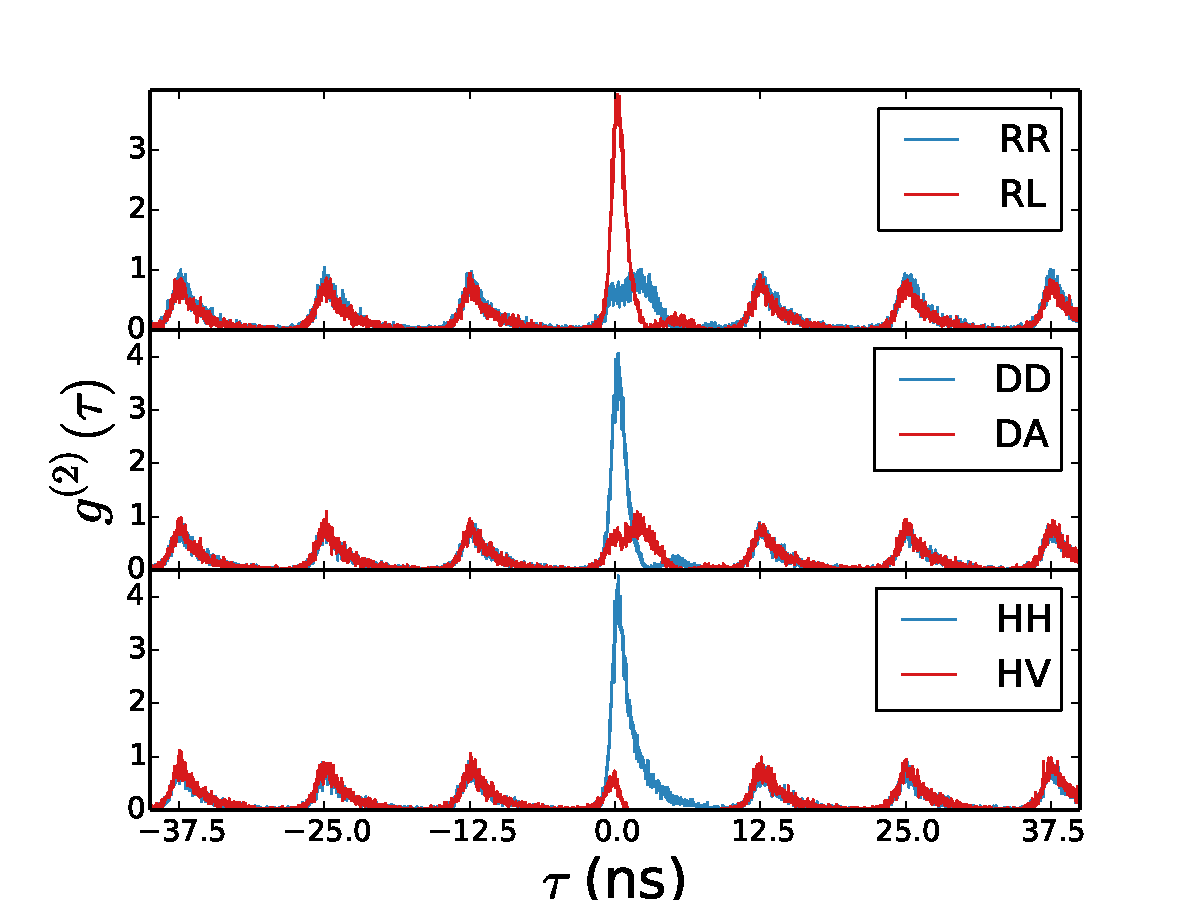
\includegraphics[width=0.7\textwidth]{images/correlations.pdf}
    \caption{Monte Carlo simulated correlation curves in the linear, diagonal and circular bases.}
    \label{fig:correlationssim}
\end{figure}

The simulation is able to recreate results for single photon
exciton-exciton auto correlation curves and exciton-biexciton
correlation curves. Presented here are the polarization resolved
biexciton-exciton curves. The parameters used are presented in Table
\ref{tab:paramstable}. A large decoherence time was chosen such that the
probability of a decoherence event occurring in the simulation was
effectively zero. This was done to clearly show the time dependence in
the correlation curves.

\begin{figure}
\centerfloat
\begin{subfigure}{.5\textwidth}
  \centering
  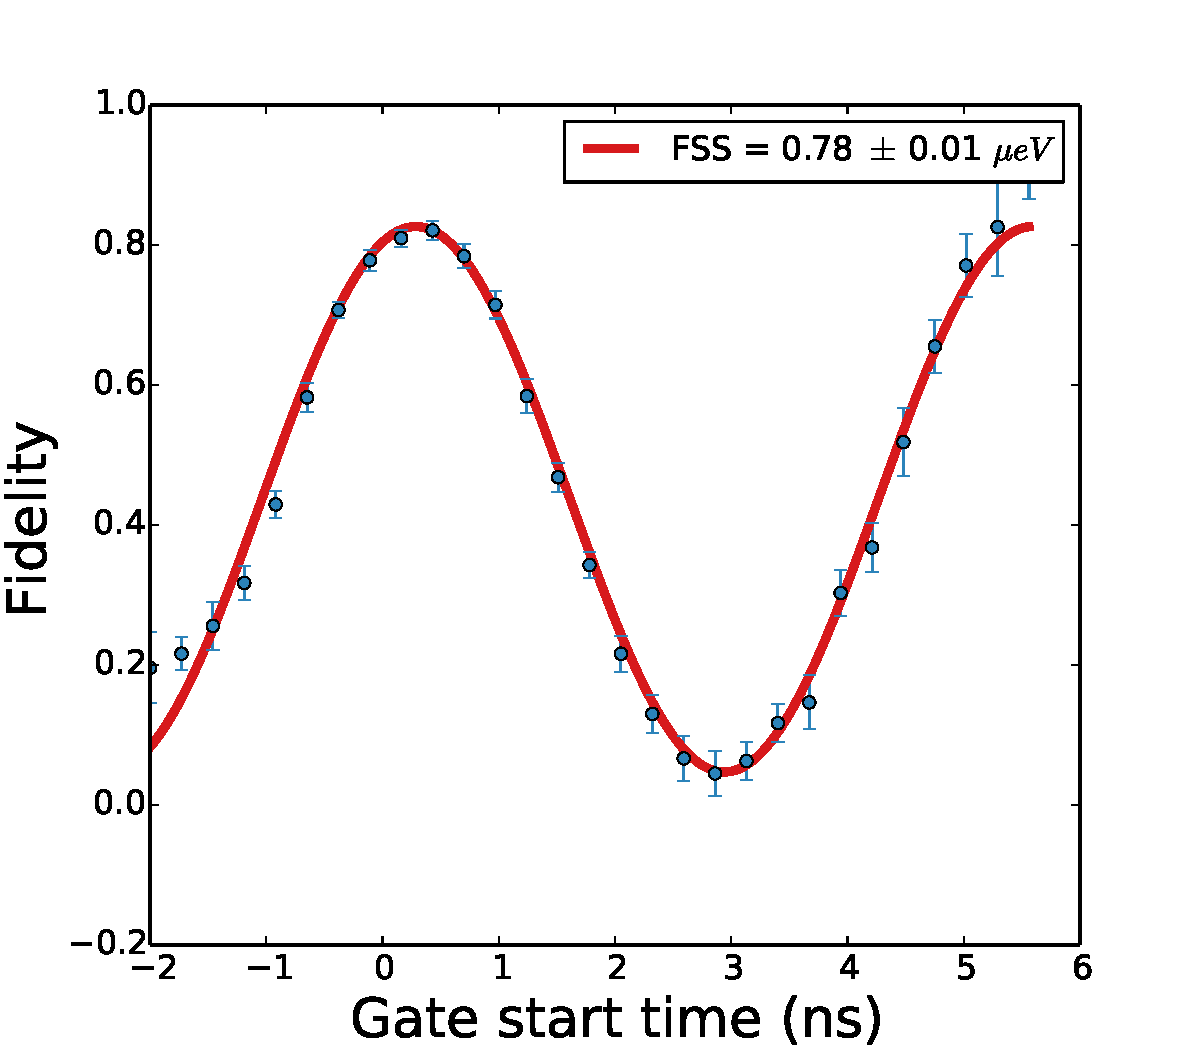
\includegraphics[width=1\linewidth]{images/fidelity_gatestart.pdf}
  \caption{}
  \label{fig:sub1}
\end{subfigure}%
\begin{subfigure}{.5\textwidth}
  \centering
  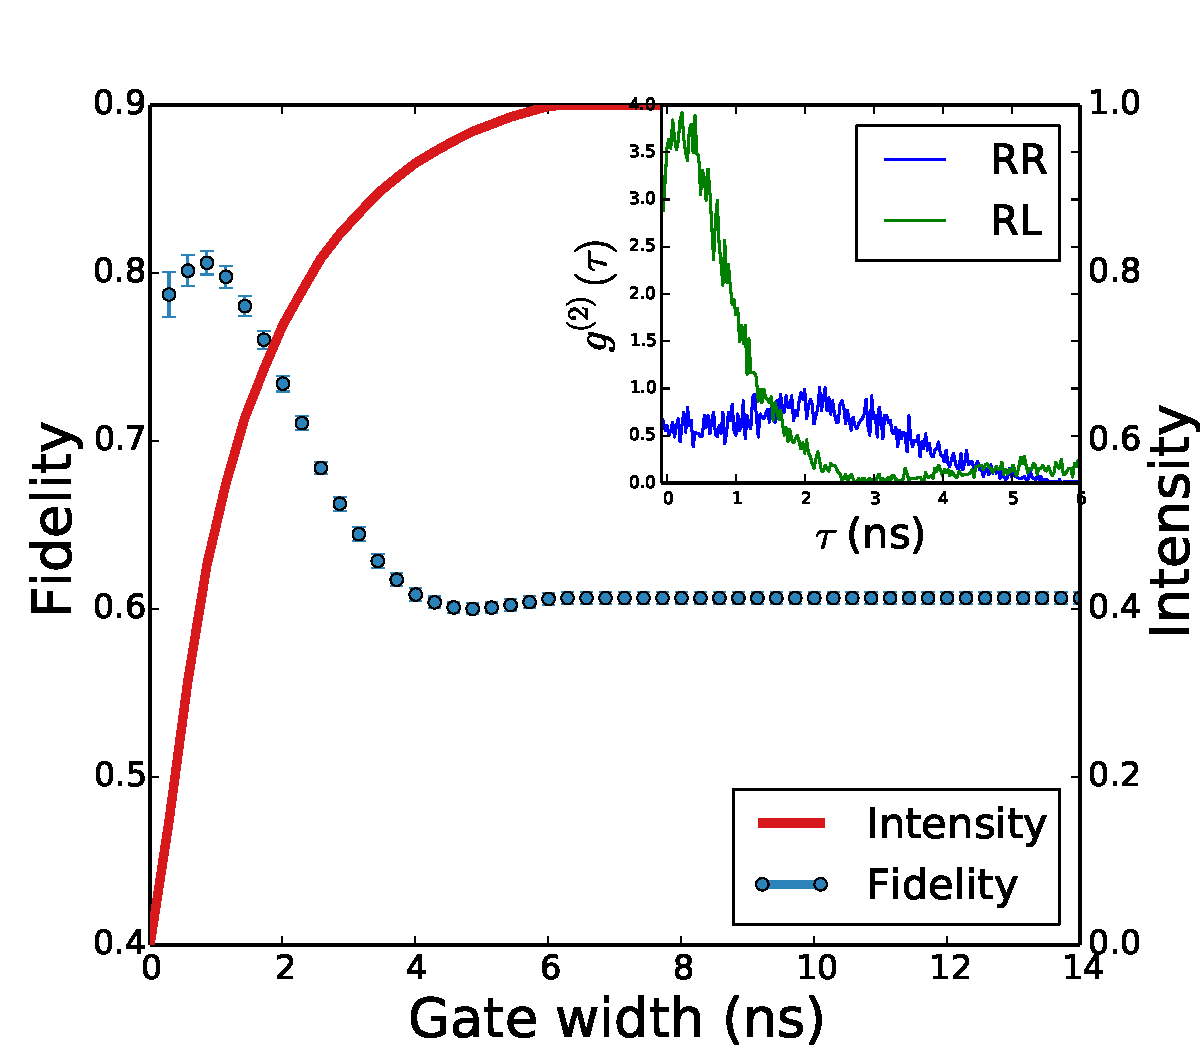
\includegraphics[width=1\linewidth]{images/fidelity_gatewidth.pdf}
  \caption{}
  \label{fig:decaypath}
\end{subfigure}
\caption{(a) Monte Carlo simulated fidelity vs gate start for a gate width of 0.2 $ns$ (b) Monte Carlo simulated fidelity vs gate width starting at 0 $ns$.}
\label{fig:timegatesim}
\end{figure}

The data from the simulated correlation curves was treated in the exact
same way as the measured correlation curves when time gated. Figure
\ref{fig:timegatesim} shows the simulated fidelity versus gate start
time and gate width. They are in very good agreement with the measured
results.

This theory of time dependent entanglement is supported by the data
presented in this chapter. It is important to understand this time
dependent entanglement when designing QD's, it gives a quantitative
measure on how the FSS and the exciton, biexciton lifetimes will
influence measured entanglement. Making the FSS and lifetimes smaller is
the preferable approach.

This theory could potentially be used to allow fine control of the phase
of the emitted photonic state. Pre-selection in time of the emitted
photons would be quite useful as opposed to the post-selection presented
in this work. This phase selection comes at a cost of intensity, however
this may be compensated by having suitably efficient collection.
\newpage

\section{Charged biexciton states}

This chapter concerns the identification of a specific excitonic pattern
present in the QDs emitting entangled photons. This work was done by the
author and Dr.~Gediminas Juska, both took measurements, while Dr.~Juska
developed the theory and the author worked on the mathematical modeling.

\subsection{Theory}\label{theory}

A constant feature of the QDs reported by the EPN group in Ref
\cite{gjnature} and presented in Chapter 3 of this work is a typical
spectrum for the entangled photon emitting QD's. It is seen that there
is two distinct spectrum on the sample. One of which consistently (
$\sim$ 75\%) passes entanglement tests, and one which always fails. In
this chapter a detailed analysis was done on the entangled photon
emitting pattern, shown in Figure \ref{fig:trionspectrum}. As will be
discussed, it is hypothesised that the population of these QDs is
dominated by positively charged carriers. A describing fine structure is
tentatively presented and then data and models are presented to
reinforce the theory \cite{self}.

\begin{figure}[h!]
    \centering
    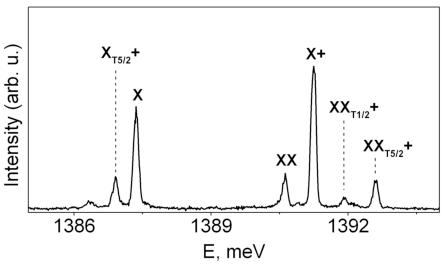
\includegraphics[width=0.6\textwidth]{images/trionspectrum.pdf}
    \caption[]{Typical spectrum of QDs which pass entanglement tests. \protect\footnotemark}
    \label{fig:trionspectrum}
\end{figure}

\footnotetext{Courtesy of Dr. Juska}

A trion is an exciton which has a surplus electron or hole, a hot trion
is when the surplus carrier is in the excited state. It is assumed that
this charged environment is an independent product of whatever growth
process creates these highly symmetric QDs and that the pattern is not
in itself an inherent properties highly symmetric dots. Unambiguous
identification of whether the excitonic species was positively or
negatively charged was not made in the scope of this work. A QD
light-emitting diode structure \cite{baierdiode} is a strategy for
identification of whether the QD charging is positive or negative. This
LED structure is under preliminary development for pyramidal QDs and was
unavailable at this time. Thus the identification of the charging
environment as positive is based on equivalence with literature (Review.
\cite{review}). Theoretically there is no limit on the energetic
structure of different charging configurations however it is typically
reported that positive QDs are at higher energy than neutral, and the
negative QDs are at lower energy.

\begin{figure}[h!]
    \centering
    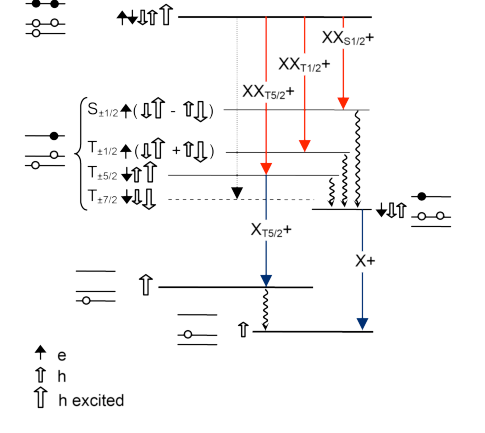
\includegraphics[width=0.6\textwidth]{images/trionfinestructure.pdf}
    \caption[]{Energetic structure of the biexciton \protect\footnotemark}
    \label{fig:trionfinestructure}
\end{figure}

\footnotetext{Courtesy of Dr. Juska}

The theorised fine structure of charged biexciton system is depicted in
Figure \ref{fig:trionfinestructure} \cite{ht1, ht2, ht3}. The
recombination from the initial charged biexciton state is complicated by
the fine-structure of the hot trion. According to Kramers theorem, an
energy level with half-integer spin is at least doubly degenerate, the
initial charged biexciton state ($\pm$ 3/2) is double degenerate. It
decays to a hot trion, one electron and two holes -- one ground hole and
the other excited. The hot trion has eight possible total spin
configurations resulting in eightfold degeneracy. The hole-hole exchange
interaction causes the splitting of the energetic level to a double
degenerate singlet state ($\pm 1/2$) and a six-fold triplet state.
Electron-hole exchange interaction causes a further splitting of the
triplet states. The resulting energy fine-structure has four double
degenerate levels \cite{ht2}. The singlet state $S_{\pm 1/2}$ is the
highest energy state followed by $T_{\pm 1/2}$, $T_{\pm 5/2}$ and
$T_{\pm 7/2}$.

Identification of the transitions was carried out by excitation power
dependent and photon cross-correlations measurements and a theoretical
QD population model. The typical spectrum shown in Figure
\ref{fig:trionspectrum} was made up of transitions that originated from
two recombination cascades -- the neutral biexciton-exciton cascade and
that of the positively charged biexciton-excited trion. A populated
charged biexciton decays optically to the three doubly degenerate hot
trion states. These transitions are observed as $XX_{S1/2+}$,
$XX_{T1/2+}$ and $XX_{T5/2+}$ in the spectrum. Transition to the
$T_{\pm7/2}$ state is forbidden by optical recombination. The singlet
$S_{\pm1/2}$ and the triplet $T_{\pm1/2}$ states are believed to be very
short living and decay to the ground trion as the excited hole very
rapidly relaxes to the ground level \cite{ht2, ht3}. The state
$T_{\pm5/2}$ is composed of a ground hole and excited hole that have the
same spin, thus the excited hole relaxation to the ground level is
restricted by Pauli exclusion principle. If the hole spin flip rate
$\gamma_{sf}$ is comparable to the spontaneous recombination rate then
this state can recombine optically, this is transition $X_{T5/2+}$ in
the spectrum.

\subsection{Experimental and
modelling}\label{experimental-and-modelling}

Photon correlation measurements taken in a continuous-wave excitation
mode allowed the identification of the cascade order of the transitions.
These measured second order correlation $g^{(2)}(\tau)$ curves are shown
in Figure \ref{fig:trioncorrs}. On the positive time scale the second
order correlation function represents the probability of detecting a
photon emitted by transition $T_n$ being followed by a photon emitted by
a transition $T_m$. On the negative timescale the opposite is true
($T_m$ being followed by $T_n$). For example there should be an
increased probability of an $XX$ photon being followed by an $X$ photon
and decreased probability of the reverse occurring (Top image in Figure
\ref{fig:trioncorrs}).

\begin{figure}[H]
    \centering
    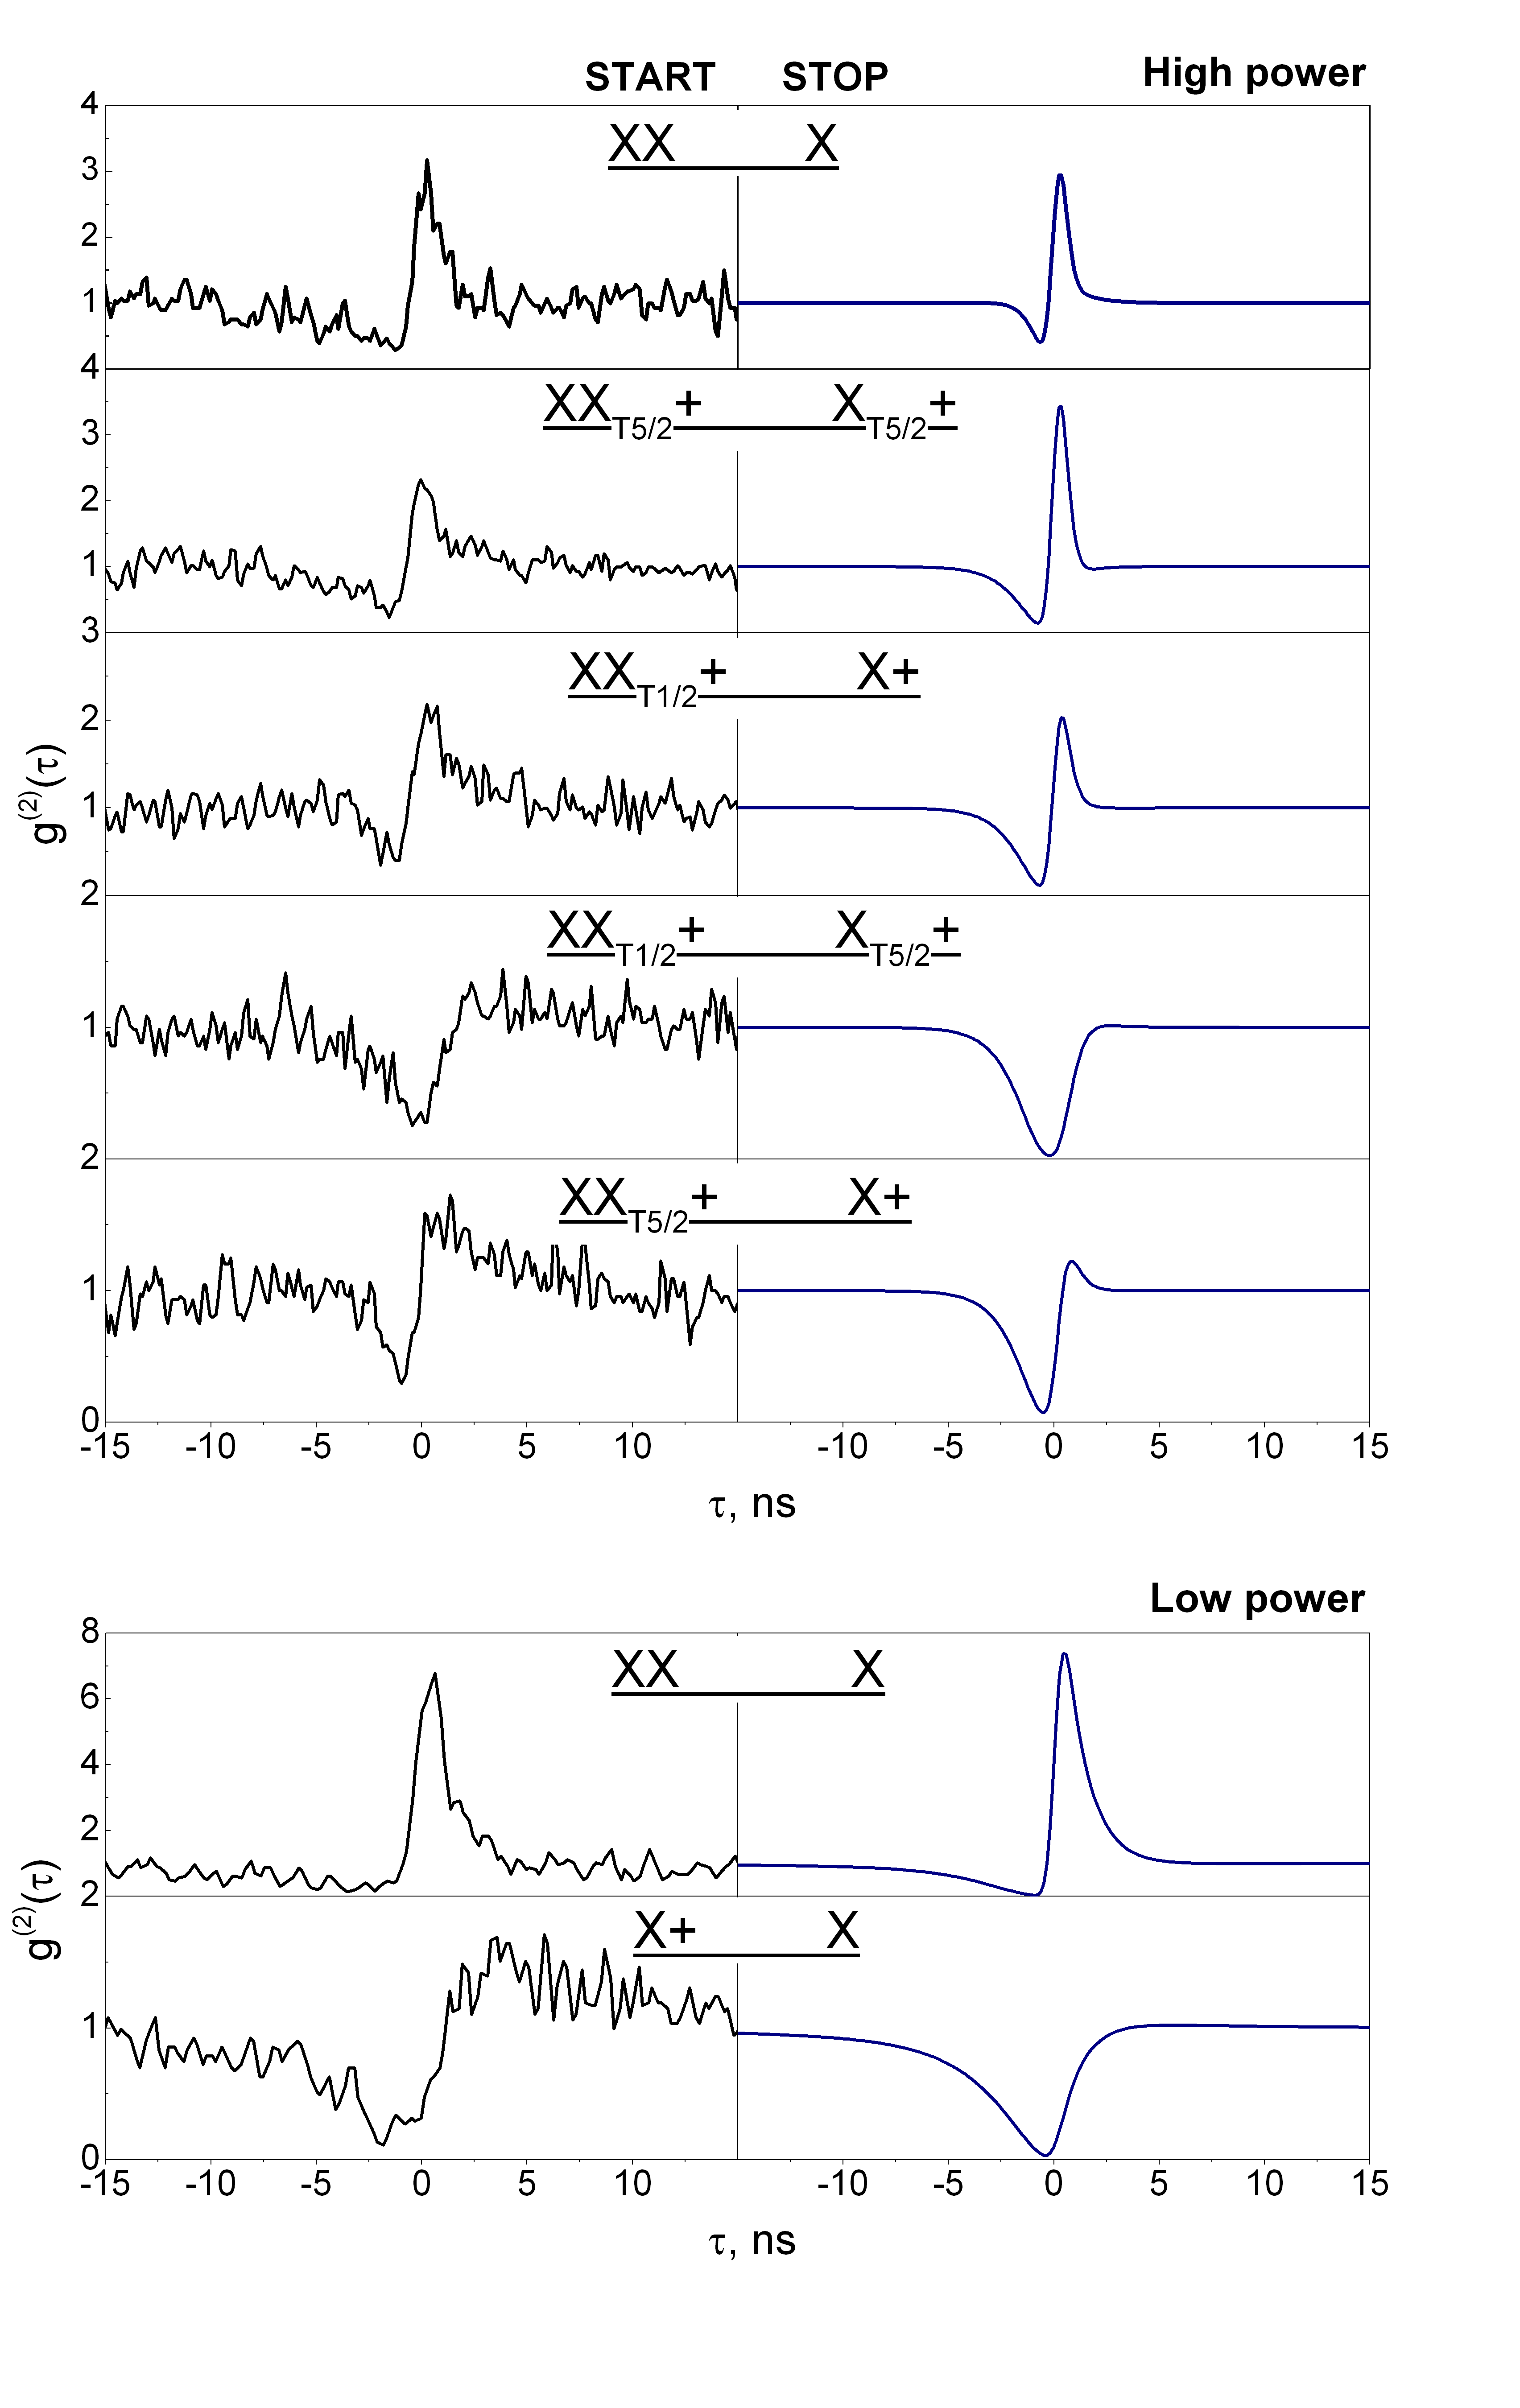
\includegraphics[width=0.5\textwidth]{images/ABcoeff.png}
    \caption{Measured and theoretical correlations curves for different transition pairs. }
    \label{fig:trioncorrs}
\end{figure}

A rate equation model was developed to analyse the correlation curves.
This model was based on the theory of random population presented in Ref
\cite{grundmann} and charged excitonic model in Ref \cite{baiermodel}.
The model presented here includes also excited excited states (and
excludes negative states). The probability of being in a given state
$p_{it}(t)$ depends on the rates at which one enters and exits the
state. A state is populated by capturing electrons and holes with
characteristic times $t_e$ and $t_h$, or by decaying into the state
$p_{it}(t)$ from a transition cascade. A state exits by decaying
optically with characteristic lifetime $\tau_{ij}$ or by moving to
another state by electron or hole capture.

In general the rate of change of the state probability is given by

\begin{equation}
\frac{d \bar{P}}{dt} = A \bar{P}
\end{equation}

Where $A$ is a transition matrix made up of the rate of entering and
exiting a state. The rate equations are presented here

\begin{align}
\frac{d p_{000}}{dt}&= \frac{p_{101}}{\tau_{101}} - \frac{p_{000}}{t_h}        - \frac{p_{000}}{t_e}, \\[5pt]
\frac{d p_{100}}{dt}&= \frac{p_{000}}{t_h}       + \frac{p_{201}}{\tau_{201}} - p_{100}\frac{c_e}{t_e} - p_{100}\frac{c_h}{t_h} + \frac{p_{010}}{\tau_{010}},\\[5pt]
\frac{d p_{200}}{dt}&= p_{100}\frac{c_h}{t_h}     - p_{200}\frac{c_e}{t_e},\\[5pt]
\frac{d p_{001}}{dt}&= \frac{p_{000}}{t_e}        - p_{001}\frac{d_h}{t_h},\\[5pt]
\frac{d p_{010}}{dt}&= \frac{p_{111}}{\tau_{111}} - \frac{p_{010}}{\tau_{010}},\\[5pt]
\frac{d p_{101}}{dt}&= p_{100}\frac{c_e}{t_e}     + p_{001}\frac{d_h}{t_h}    + \frac{p_{202}}{\tau_{202}} - \frac{p_{101}}{\tau_{101}}- \frac{p_{101}}{t_h},\\[5pt]
\frac{d p_{111}}{dt}&= \frac{2}{3}\frac{p_{212}}{\tau_{212T5/2}}              + \frac{1}{2}\frac{p_{101}}{t_h} - \gamma_{sf}p_{111} - \frac{p_{111}}{\tau_{111}},\\[5pt]
\frac{d p_{201}}{dt}&= \frac{1}{2}\frac{p_{101}}{t_h} + p_{200}\frac{c_e}{t_e}+ \frac{1}{3}\frac{p_{212}}{\tau_{212T1/2}} + \gamma_{sf}p_{111} - p_{201}\frac{c_e}{t_e} + \frac{p_{201}}{\tau_{201}},\\[5pt]
\frac{d p_{202}}{dt}&= p_{201}\frac{c_e}{t_e}     - \frac{p_{202}}{\tau_{202}}- \frac{p_{202}}{t_h},\\[5pt]
\frac{d p_{212}}{dt}&= \frac{p_{202}}{t_h}        - \frac{1}{3}\frac{p_{212}}{\tau_{212T1/2}} - \frac{2}{3}\frac{p_{212}}{\tau_{212T5/2}},\\[5pt]
\sum_ip_i(t)&= 1 
\end{align}

Where $p_{abc}$ is the probability of being in state with $a$ holes, $b$
excited holes and $c$ electrons. $\tau_{abc}$ is the decay time of state
with $a$ holes, $b$ excited holes and $c$ electrons. Where $\gamma_{sf}$
is the excited hole spin flip time. $t_e$ ($t_h$) is the electron (hole)
capture time and $c_e$, $c_h$, $d_e$, $d_h$ are Coulomb coefficients as
explained below. These equations are represented schematically in Figure
\ref{fig:rateequationscheme}. Red arrows represent radiative
recombination and the measurable emission of a photon. The radiative
lifetimes $\tau_{ij}$ were measured and used directly in the modeling.

A $g^{(2)}(\tau)$ curve was modeled by plotting on the positive
timescale $p_{i}(t)$ which decays to state $p_j(t)$ with the initial
condition of being in whatever state populates state $i$, and $p_{j}(t)$
with initial condition of being in the state $j$ on the negative
timescale.

\begin{figure}[H]
    \centering
    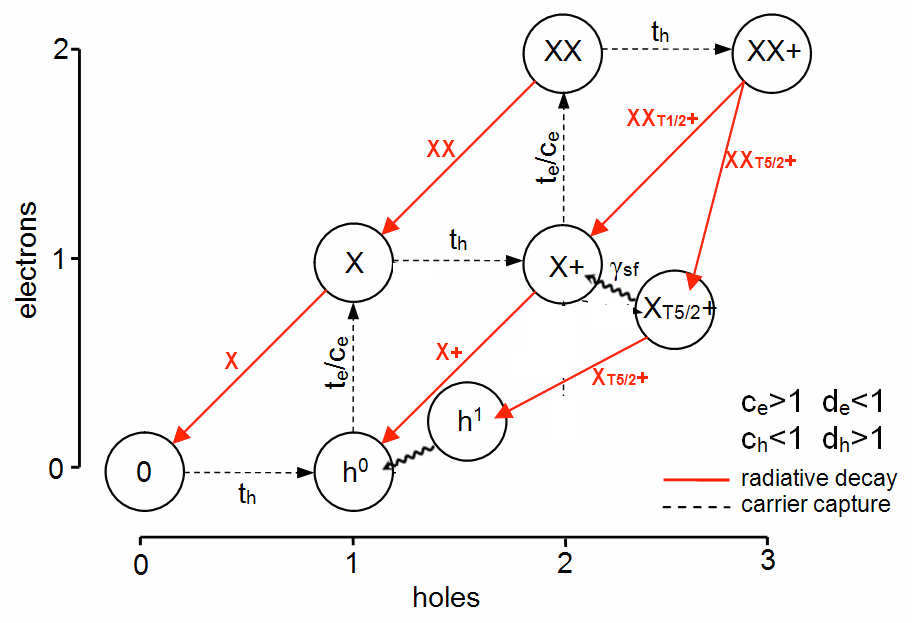
\includegraphics[width=0.65\textwidth]{images/s.png}
    \caption{Schematic of the rate equations used model the measured correlations.}
    \label{fig:rateequationscheme}
\end{figure}

The response function of the APDs was measured to be a Gaussian and has
a FWHM of 0.71ns. The model accounted for this by numerically
convoluting the rate equations with this response function. Coulomb
interactions were included in the model. These interactions occur when
the QD is populated by a charged complexes, for example electron capture
is faster when the QD is positively charged. The corrections modify the
electron (hole) capture time $t_e$ ($t_h$) reducing (increasing) it by
$c_e$ ($c_h$) when a QD is positively charged and increasing (reducing)
it by $d_e$ ($d_h$) when charging is negative. Since the QD is
negatively charged in only one instance, when it is populated by an
electron, the term $d_e$ never comes into play and $d_h$ is included
only didactically. The following simplifications were made in the model.
In the spectrum shown in Figure \ref{fig:trionspectrum}, only the two
transitions $XX_{T1/2+}$ and $XX_{T5/2+}$ from the charged biexciton to
the triplet states were clearly observed. The relaxation of the hot
trion state $X_{T1/2+}$ to the ground trion $X_+$ is reported to be very
rapid \cite{ht3}, on the order of picoseconds which is ignored on the
scale of the model which is nanoseconds. Thus in the model the state
$X_{T1/2+}$ was considered equivalent to the state $X_{+}$. The state
$X_{T5/2+}$ needs a spin flip in order to decay to $X_+$. Thus it lives
longer. A hole spin flip term $\gamma_{sf}$ was included in the state
$X_{T/2+}$ equation, similarly to Ref. \cite{ht3}.

The fitting to the experimental data was done quite strictly with the
only free parameters being the coulomb terms $c_e$ and $c_h$, the
electron and hole capture times $t_e$ and $t_h$, the hole relaxation
time $\tau_{001}$ and the spin flip time $\gamma_{sf}$. This is in
contrast to similar models where the radiative lifetimes are not set
parameters. The small discrepancies between te model and experiment can
be explained by the complexity of the system and the measurement
procedure. The fittings assume that the parameters are constant
throughout the whole measurement, which is unlikely in practice as the
experiment typically takes a few hours. Sample drifting and power
fluctuations would have the effect of slightly modifying the measurement
conditions over time. There is a good overall agreement between the
fittings and the data, especially since the same model was used to
describe the high and low power measurements. The spin flip time
$\gamma_{sf}$ of the excited hole was calculated to be 1.8ns$^{-1}$
(0.55ns) which is of the same scale as the radiative lifetime of the
$X_{T5/2+}$ state. The electron capture time $t_e$ was found to be
1.03ns and the hole capture time $t_h$ was found to be 0.38ns. This
smaller hole capture time is consistent with the positively dominated
excitonic system.

\newpage
\section{Conclusions and further work}

This report has been a summary of work done to categorise and fully
understand the entangled photon emitting QDs.

Chapter 3 was concerned with understanding the time evolution of the
polarisation entanglement. Using the time gating theory a dramatic rise
in the entanglement fidelity was achieved. This theory is important both
for understanding the underlying dynamics of the biexciton-exciton
entangled cascade and also as a technique to achieve higher fidelity in
a regime where time discrimination is possible. There may also be use
cases in time-dependent quantum logic, where the phase of the entangled
state may be chosen.

Chapter 4 presented a detailed study on the excitonic pattern observed
in the QDs which have a high propensity for entangled photon emission. A
theoretical model was developed and was seen to have good agreement with
the measurements. Further work has been done in this area by the group
since the end of this project. It has been seen that the second
excitonic patterns seen on the sample are likely to be negatively
charged. This implies that the entangled photon emission from the second
pattern may only be practically useless, because the exciton intensity
is so low. This negative charging has the ability to be tuned by adding
a second excitation wavelength (around 1 $\mu m$) which allowed gradual
tuning of the QD from positive to negative. This tuning has the
potential to greatly increase the density of entangled photon emitters.

Further work would include investigating the QDs under resonant
excitation, where the exciton and biexciton states are populated
directly. With this neutral excitation the quality of the spectrum and
the entanglement may improve. The group is also now focusing on
different tuning strategies for the QDs. QDs integrated on piezoelectric
crystals can be tuned through strain has been shown by the group to
alter the wavelength through a free meV. The FSS has been shown to be
tunable by a vertical electric field \cite{verfield}.

\newpage
\section{Appendix 1}

The HWP matrix adapted to the lab basis is give by:

\[ HWP = \begin{pmatrix}
            & hwp(\theta_x)& 0& 0& 0& 0& 0& 0 \\
            & & 0& 0& 0& 0& 0& 0 \\
            0& 0& hwp(\theta_x)& & 0& 0& 0& 0 \\
            0& 0& & & 0& 0& 0& 0 \\
            0& 0& 0& 0&hwp(\theta_{xx}) & & 0& 0 \\
            0& 0& 0& 0& & & 0& 0 \\
            0& 0& 0& 0& 0& 0&hwp(\theta_{xx}) &  \\
            0& 0& 0& 0& 0& 0& & \\
            \end{pmatrix}\]

Where $hwp$ is
\[hwp = \begin{pmatrix} \cos{2 \theta} & \sin{2 \theta} \\ \sin{2 \theta} & -\cos{2 \theta} \end{pmatrix}\]

The QWP matrix adapted to the lab basis is give by:

\[ QWP = \begin{pmatrix}
            & qwp(\theta_x)& 0& 0& 0& 0& 0& 0 \\
            & & 0& 0& 0& 0& 0& 0 \\
            0& 0& qwp(\theta_x)& & 0& 0& 0& 0 \\
            0& 0& & & 0& 0& 0& 0 \\
            0& 0& 0& 0&qwp(\theta_{xx}) & & 0& 0 \\
            0& 0& 0& 0& & & 0& 0 \\
            0& 0& 0& 0& 0& 0&qwp(\theta_{xx}) &  \\
            0& 0& 0& 0& 0& 0& & \\
            \end{pmatrix}\]

Where $qwp$ is
\[qwp = \begin{pmatrix} 1 + i \cos{2 \theta} & i \sin{2 \theta} \\ i \sin{2 \theta} & 1- i \cos{2 \theta} \end{pmatrix}\]

Here we present the mappings made for the optical bench apparatus.

For the neutral beam splitter ($NBS$) this operator is given by making
the mapping:

\[ NBS \left| \psi \hat{i} \right\rangle = \frac{1}{\sqrt{2}}( \left| \psi \hat{i} \right\rangle + \left| \psi \hat{j} \right\rangle )\]
\[ NBS \left| \psi \hat{j} \right\rangle = \frac{1}{\sqrt{2}}( \left| \psi \hat{i} \right\rangle + \left| \psi \hat{j} \right\rangle )\]

Where $\left| \psi \hat{i} \right\rangle$ is a state moving in the
$\hat{i}$ direction. With matrix

\[NBS = \frac{1}{\sqrt{2}}\begin{pmatrix}
1 & 0 & 1 & 0& 0& 0& 0& 0\\0& 1& 0& 1& 0& 0& 0& 0\\1& 0& 1& 0& 0& 0& 0& 0\\0& 1& 0& 1& 0& 0& 0& 0\\0& 0& 0& 0& 1& 0& 1& 0\\0& 0& 0& 0& 0& 1& 0& 1\\0& 0& 0& 0& 1& 0& 1& 0\\0& 0& 0& 0& 0& 1& 0& 1\end{pmatrix}\]

In general beam splitters impart a phase rotation on the reflected
state, however a phase difference in the positional degree of freedom is
not measured in the simulation. It was tested and seen to not make any
difference in the results of the simulation. The polarising beam
splitter ($PBS$) is given by making the mappings:

\[ PBS \left| \hat{i} \ \hat{h} \ \hat{e}_{xx} \right\rangle = \left| \hat{i} \ \hat{h} \ \hat{e}_{xx}  \right\rangle\]

\[ PBS \left| \hat{i} \ \hat{v} \ \hat{e}_{xx} \right\rangle = \left| \hat{j} \ \hat{h} \ \hat{e}_{xx}  \right\rangle\]

\[ PBS \left| \hat{i} \ \hat{h} \ \hat{e}_{x} \right\rangle = \left| \hat{i} \ \hat{h} \ \hat{e}_{x}  \right\rangle\]

\[ PBS \left| \hat{i} \ \hat{v} \ \hat{e}_{x} \right\rangle = \left| \hat{j} \ \hat{h} \ \hat{e}_{x}  \right\rangle\]

\[ PBS \left| \hat{j} \ \hat{h} \ \hat{e}_{xx} \right\rangle = \left| \hat{j} \ \hat{h} \ \hat{e}_{xx} \right\rangle\]

\[ PBS \left| \hat{j} \ \hat{v} \ \hat{e}_{xx} \right\rangle = \left| \hat{i} \ \hat{h} \ \hat{e}_{xx} \right\rangle\]

\[ PBS \left| \hat{j} \ \hat{h} \ \hat{e}_{x} \right\rangle = \left| \hat{j} \ \hat{h} \ \hat{e}_{x} \right\rangle\]

\[ PBS \left| \hat{j} \ \hat{v} \ \hat{e}_{x} \right\rangle = \left| \hat{i} \ \hat{h} \ \hat{e}_{x} \right\rangle\]

With matrix

\[PBS = \begin{pmatrix} 1& 0& 0& 0& 0& 0& 0& 0\\0& 0& 0& 1& 0& 0& 0& 0\\0& 0& 1& 0& 0& 0& 0& 0\\0& 1& 0& 0& 0& 0& 0& 0\\0& 0& 0& 0& 1& 0& 0& 0\\0& 0& 0& 0& 0& 0& 0& 1\\0& 0& 0& 0& 0& 0& 1& 0\\0& 0& 0& 0& 0& 1& 0& 0 \end{pmatrix}\]
The $\hat{e}_x$ monochromator ($S_x$) workes by only allowing energy
$\hat{e}_x$ through and is given by making the mappings:

\[ S_x \left| \hat{i} \ \hat{h} \ \hat{e}_{xx} \right\rangle = \left| \hat{i} \ \hat{h} \ \hat{e}_{xx}  \right\rangle\]

\[ S_x \left| \hat{i} \ \hat{v} \ \hat{e}_{xx} \right\rangle = \left| \hat{i} \ \hat{h} \ \hat{e}_{xx}  \right\rangle\]

\[ S_x \left| \hat{i} \ \hat{h} \ \hat{e}_{x} \right\rangle = \left| 0  \right\rangle\]

\[ S_x \left| \hat{i} \ \hat{v} \ \hat{e}_{x} \right\rangle = \left| 0  \right\rangle\]

The $\hat{e}_{xx}$ monochromator ($S_{xx}$) workes by only allowing
energy $\hat{e}_{xx}$ through and is given by making the mappings:

\[ S_{xx} \left| \hat{j} \ \hat{h} \ \hat{e}_{xx} \right\rangle = \left| 0 \right\rangle\]

\[ S_{xx} \left| \hat{j} \ \hat{v} \ \hat{e}_{xx} \right\rangle = \left| 0 \right\rangle\]

\[ S_{xx} \left| \hat{j} \ \hat{h} \ \hat{e}_{x} \right\rangle = \left| \hat{j} \ \hat{h} \ \hat{e}_{x} \right\rangle\]

\[ S_{xx} \left| \hat{j} \ \hat{v} \ \hat{e}_{x} \right\rangle = \left| \hat{j} \ \hat{h} \ \hat{e}_{x} \right\rangle\]

The monochromator matrix $S$ is given by the sum of $S_x$ and $S_{xx}$.

\[S = \begin{pmatrix} 0& 0& 0& 0& 0& 0& 0& 0\\0& 0& 0& 0& 0& 0& 0& 0\\0& 0& 1& 0& 0& 0& 0& 0\\0& 0& 0& 1& 0& 0& 0& 0\\0& 0& 0& 0& 1& 0& 0& 0\\0& 0& 0& 0& 0& 1& 0& 0\\0& 0& 0& 0& 0& 0& 0& 0\\0& 0& 0& 0& 0& 0& 0& 0 \end{pmatrix}\]

\newpage

\addcontentsline{toc}{section}{References}

\begin{thebibliography}{99}

\bibitem{self}
  G. Juska, \textbf{E. Murray}, V. Dimastrodonato, T. H. Chung, A. Gocalinska \& E. Pelucchi
  \emph{Entangled photon emission from (111)B site-controlled Pyramidal quantum dots.}
  Submitted to Phys. Rev. B.
  (2014).

\bibitem{self2}
  \textbf{E. Murray}, G. Juska, \& E. Pelucchi
  \emph{Monte Carlo simulation suite for various Quantum dot experiments}
  (In production).

\bibitem{github}
  \textbf{E. Murray},
  \emph{ \url{http://www.github.com/eoinmurray/icarus2} }
  Accessed on 3rd April 2014.

\bibitem{first}
  Oliver Benson, Charles Santori, Matthew Pelton, \& Yoshihisa Yamamoto.
  \emph{Regulated and Entangled Photons from a Single Quantum Dot.}
  Phys. Rev. Lett.
  84,
  2513 (2000).

\bibitem{gjnature}
  G. Juska, V. Dimastrodonato, L. O. Mereni, A. Gocalinska \& E. Pelucchi.
  \emph{Towards quantum-dot arrays of entangled photon emitters}.
  Nature Photonics 
  7, 
  527–531 (2013).

\bibitem{bible}
   M. A. Nielsen \& I. L. Chuang.
   \emph{Quantum Computation and Quantum Information. Chapter 2.}
   Cambridge University Press (2000). 

\bibitem{fox}
    M. Fox
   \emph{Quantum Optics, an introduction. Chapter 6.}
   Oxford University Press (2006). 

\bibitem{jones}
  R. C. Jones.
  \emph{A new calculus for the treatment of optical systems, I. Description and Discussion of the Calculus.}
  Jour. Optical Society of America,
  31, 
  (7) 488–493 (1941).

\bibitem{jones1}
  G. Fowles.
  \emph{Introduction to Modern Optics (2nd ed.).}
  Dover (1989),
  p. 35.

\bibitem{jones2}
  A. Gerald \& J. M. Burch.
  \emph{Introduction to Matrix Methods in Optics (1st ed.).} 
  John Wiley \& Sons.
  (1975)

\bibitem{rioux}
  F. Rioux
  \emph{ \url{http://www.users.csbsju.edu/\textasciitildefrioux/photon/MZ-Polarization.pdf} }
  Accessed on 3rd April 2014.

\bibitem{ry1}
  R. M. Stevenson, R. J. Young, P. See, D. G. Gevaux, K. Cooper, P. Atkinson, I. Farrer, D. A. Ritchie \& A. J. Shields. 
  \emph{Magnetic field induced reduction of fine structure splitting in quantum dots.}
  Phys. Rev. B 
  73, 
  033306 (2006).

\bibitem{ry2}
  R. J. Young, R. M. Stevenson, A. J. Shields, P. Atkinson, K. Cooper, D. A. Ritchie, K. M. Groom, A. I. Tartakovskii, \& M. S. Skolnick.
  \emph{Inversion of the exciton fine structure splitting in quantum dots.} Physica E 
  32, 
  97 (2006)

\bibitem{entangletime}
  R. Mark Stevenson, Andrew J. Hudson, Anthony J. Bennett, Robert J. Young, Christine A. Nicoll, David A. Ritchie, Andrew J. Shields.
  \emph{Evolution of Entanglement Between Distinguishable Light States. }
  Phys. Rev. Lett. 
  101, 
  170501 (2008).

\bibitem{hudson}
  A. J. Hudson, R. M. Stevenson, A. J. Bennett, R. J. Young, C. A. Nicoll, P. Atkinson, K. Cooper, D. A. Ritchie, \& A. J. Shields.
  \emph{Coherence of an entangled exciton-photon state. }
  Phys. Rev. Lett. 
  99, 
  266802 (2007).

\bibitem{f1}
  M. Ghali, K. Ohtani, Y. Ohno \& H. Ohno.
  \emph{Generation and control of polarization- entangled photons from GaAs island quantum dots by an electric field. }
  Nat. Commun.
  3, 
  661 (2012).

\bibitem{entandiode}
  R. M. Stevenson, C. L. Salter, J. Nilsson, A. J. Bennett, M. B. Ward, I. Farrer, D. A. Ritchie, \& A. J. Shields
  \emph{Indistinguishable Entangled Photons Generated by a Light- Emitting Diode.}
  Phys. Rev. Lett.
  108, 
  040503  (2012).

\bibitem{amotomo}
  D. F. V. James, P. G. Kwiat, W. J. Munro, and A. G. White
  \emph{Measurement of qubits. }
  Phys. Rev. A 
  64, 
  052312 (2001).

\bibitem{review}
  A. Schliwa, M. Winkelnkemper, \& D. Bimberg.
  \emph{Few-particle energies versus geometry and composition of $\text{In}_x\text{Ga}_{1-x}\text{As/GaAs}$ self-organized quantum dots}
  Phys. Rev. B 
  79, 
  075443 (2009).

\bibitem{baierdiode}
  M. Baier, F. Findeis, A. Zrenner, M. Bichler, \& G. Abstreiter.
  \emph{Optical spectroscopy of charged excitons in single quantum dot photodiodes}.
  Phys. Rev. B 
  64, 
  195326 (2001).

\bibitem{ht1}
  E. Poem, J. Shemesh, I. Marderfeld, D. Galushko, N. Akopian, D. Gershoni, B. D. Gerardot, A. Badolato, \& P. M. Petroff. 
  \emph{Polarization sensitive spectroscopy of charged quantum dots.}
  Phys. Rev. B 
  76, 
  235304 (2007).

\bibitem{ht2}
  T. Warming, E. Siebert, A. Schliwa, E. Stock, R. Zimmermann, \& D. Bimberg.
  \emph{Hole-hole and electron-hole exchange interactions in single InAs/GaAs quantum dots.}
  Phys. Rev. B 
  79, 
  125316 (2009).
  
\bibitem{ht3}
  Y. Igarashi, et al.
  \emph{Spin dynamics of excited trion states in a single InAs quantum dot.}
  Phys. Rev. B 
  81, 
  245304 (2010).

\bibitem{baiermodel}
  M. H. Baier, A. Malko, E. Pelucchi, D. Y. Oberli, \& E. Kapon. 
  \emph{Quantum-dot exciton dynamics probed by photon-correlation spectroscopy.}
  Phys. Rev. B 
  73, 
  205321 (2006).

\bibitem{grundmann}
  M. Grundmann \& D. Bimberg. 
  \emph{Theory of random population for quantum dots.}
  Phys. Rev. B 
  55, 
  9740 (1997).

\bibitem{verfield}
  A. J. Bennett, M. A. Pooley, Y. Cao, N. Sköld, I. Farrer, D. A. Ritchie \& A. J. Shields.
  \emph{Voltage tunability of single-spin states in a quantum dot.}
  Nature Commun., 
  4, 
  1522 (2013)

\end{thebibliography}
\end{document}